\documentclass[a4paper,11pt,twoside]{report}
% THIS FILE SHOULD BE COMPILED BY pdfLaTeX

% ----------------------   PREAMBLE PART ------------------------------

% ------------------------ ENCODING & LANGUAGES ----------------------

\usepackage[utf8]{inputenc}
%\usepackage[MeX]{polski} % Not needed unless You have a name with polish symbols or sth
\usepackage[T1]{fontenc}
\usepackage[english, polish]{babel}
\usepackage{longtable}
\usepackage{ltablex}
\usepackage{amsmath, amsfonts, amsthm, latexsym} % MOSTLY MATHEMATICAL SYMBOLS

\usepackage[final]{pdfpages} % INPUTING TITLE PDF PAGE - GENERATE IT FIRST!
%\usepackage[backend=bibtex, style=verbose-trad2]{biblatex}

% ---------------- MARGINS, INDENTATION, LINESPREAD ------------------

\usepackage[inner=20mm, outer=20mm, bindingoffset=10mm, top=25mm, bottom=25mm]{geometry} % MARGINS


\linespread{1.5}
\allowdisplaybreaks         % ALLOWS BREAKING PAGE IN MATH MODE

\usepackage{indentfirst}    % IT MAKES THE FIRST PARAGRAPH INDENTED; NOT NEEDED
\setlength{\parindent}{5mm} % WIDTH OF AN INDENTATION


%---------------- RUNNING HEAD - CHAPTER NAMES, PAGE NUMBERS ETC. -------------------

\usepackage{fancyhdr}
\pagestyle{fancy}
\fancyhf{}
% PAGINATION: LEFT ALIGNMENT ON EVEN PAGES, RIGHT ALIGNMENT ON ODD PAGES 
\fancyfoot[LE,RO]{\thepage} 
% RIGHT HEADER: zawartość \rightmark do lewego, wewnętrznego (marginesu) 
\fancyhead[LO]{\sc \nouppercase{\rightmark}}
% lewa pagina: zawartość \leftmark do prawego, wewnętrznego (marginesu) 
\fancyhead[RE]{\sc \leftmark}

\renewcommand{\chaptermark}[1]{\markboth{\thechapter.\ #1}{}}

% HEAD RULE - IT'S A LINE WHICH SEPARATES HEADER AND FOOTER FROM CONTENT
\renewcommand{\headrulewidth}{0 pt} % 0 MEANS NO RULE, 0.5 MEANS FINE RULE, THE BIGGER VALUE THE THICKER RULE


\fancypagestyle{plain}{
  \fancyhf{}
  \fancyfoot[LE,RO]{\thepage}
  
  \renewcommand{\headrulewidth}{0pt}
  \renewcommand{\footrulewidth}{0.0pt}
}



% --------------------------- CHAPTER HEADERS ---------------------

\usepackage{titlesec}
\titleformat{\chapter}
  {\normalfont\Large \bfseries}
  {\thechapter.}{1ex}{\Large}

\titleformat{\section}
  {\normalfont\large\bfseries}
  {\thesection.}{1ex}{}
\titlespacing{\section}{0pt}{30pt}{20pt} 

    
\titleformat{\subsection}
  {\normalfont \bfseries}
  {\thesubsection.}{1ex}{}


% ----------------------- TABLE OF CONTENTS SETUP ---------------------------

\def\cleardoublepage{\clearpage\if@twoside
\ifodd\c@page\else\hbox{}\thispagestyle{empty}\newpage
\if@twocolumn\hbox{}\newpage\fi\fi\fi}


% THIS MAKES DOTS IN TOC FOR CHAPTERS
\usepackage{etoolbox}
\makeatletter
\patchcmd{\l@chapter}
  {\hfil}
  {\leaders\hbox{\normalfont$\m@th\mkern \@dotsep mu\hbox{.}\mkern \@dotsep mu$}\hfill}
  {}{}
\makeatother

\usepackage{titletoc}
\makeatletter
\titlecontents{chapter}% <section-type>
  [0pt]% <left>
  {}% <above-code>
  {\bfseries \thecontentslabel.\quad}% <numbered-entry-format>
  {\bfseries}% <numberless-entry-format>
  {\bfseries\leaders\hbox{\normalfont$\m@th\mkern \@dotsep mu\hbox{.}\mkern \@dotsep mu$}\hfill\contentspage}% <filler-page-format>

\titlecontents{section}
  [1em]
  {}
  {\thecontentslabel.\quad}
  {}
  {\leaders\hbox{\normalfont$\m@th\mkern \@dotsep mu\hbox{.}\mkern \@dotsep mu$}\hfill\contentspage}

\titlecontents{subsection}
  [2em]
  {}
  {\thecontentslabel.\quad}
  {}
  {\leaders\hbox{\normalfont$\m@th\mkern \@dotsep mu\hbox{.}\mkern \@dotsep mu$}\hfill\contentspage}
\makeatother



% ---------------------- TABLES AD FIGURES NUMBERING ----------------------

\renewcommand*{\thetable}{\arabic{chapter}.\arabic{table}}
\renewcommand*{\thefigure}{\arabic{chapter}.\arabic{figure}}


% ------------- DEFINING ENVIRONMENTS FOR THEOREMS, DEFINITIONS ETC. ---------------

\makeatletter
\newtheoremstyle{definition}
{3ex}%                           % Space above
{3ex}%                           % Space below
{\upshape}%                      % Body font
{}%                              % Indent amount
{\bfseries}%                     % Theorem head font
{.}%                             % Punctuation after theorem head
{.5em}%                          % Space after theorem head, ' ', or \newline
{\thmname{#1}\thmnumber{ #2}\thmnote{ (#3)}}
\makeatother

\theoremstyle{definition}
\newtheorem{theorem}{Theorem}[chapter]
\newtheorem{lemma}[theorem]{Lemma}
\newtheorem{example}[theorem]{Example}
\newtheorem{proposition}[theorem]{Proposition}
\newtheorem{corollary}[theorem]{Corollary}
\newtheorem{definition}[theorem]{Definition}
\newtheorem{remark}[theorem]{Remark}

% --------------------- END OF PREAMBLE PART (MOSTLY) --------------------------





% -------------------------- USER SETTINGS ---------------------------

\newcommand{\tytul}{System zarządzania zasobami małego laboratorium chemicznego}
\renewcommand{\title}{A System for Resources Management in a Small Chemical Laboratory}
\newcommand{\type}{Engineer} % Master OR Engineer
\newcommand{\supervisor}{dr inż. Agnieszka Jastrzębska} % TITLE AND NAME OF THE SUPERVISOR



\begin{document}
\sloppy
\selectlanguage{english}


\includepdf[pages=-]{titlepage} % THIS INPUTS THE TITLE PAGE


% ------------------ PAGE WITH SIGNATURES --------------------------------

\thispagestyle{empty}\newpage
\null

\vfill

\begin{center}
\begin{tabular}[t]{ccc}
............................................. & \hspace*{100pt} & .............................................\\
supervisor's signature & \hspace*{100pt} & author's signature
\end{tabular}
\end{center}



% ---------------------------- ABSTRACTS -----------------------------

{
\begin{abstract}

\begin{center}
\title
\end{center}

For the subject of our engeeniring thesis, we have resolved a problem of management of supplies in a small chemical laboratory. We have designed and implemented a system supporting management of resources (chemical reagents, instruments, etc.). The system keeps track of the state of resources in the laboratory, and stores the data in a database. The system has graphical user-friendly interface which facilitates displaying and modifying the gathered data. Multiple functionalities in the system allow the user to: 
\begin{itemize}
\item Classify the resource into groups
\item Assign descriptions with multimedia content to resources
\item	Define and generate reports and notifications. reports are displaying current state of resources as well as plot of activity in time, plot of demand for some resource in time, bar chart, pie chart, whereas notifications are alerts about low level of some chemical reagent, etc.
\item For each resource, store suppliers’ contact data and order new resources directly from the application
\item Predict future demand for resources based on available historical data
\end{itemize}
The implemented system is a Web Application. It consists of a client application – developed in AngularJS – and server – developed in SpringBoot Java. Elements of application exchange information using RESTful API. As per development tools, we used IntelliJ IDEA (a Java integrated development environment (IDE)).
\\

\noindent \textbf{Keywords:} Resource Management, Database, Time Series Forecast, Web Application, Java, AngularJS, SpringBoot, RESTful API, IntelliJ IDEA
\end{abstract}
}

\null\thispagestyle{empty}\newpage


{\selectlanguage{polish}
\begin{abstract}

\begin{center}
\tytul
\end{center}

Jako temat pracy inżynierskiej, rozwiązalimy problem zarządzania zasobami w małym laboratorium chemicznym. Zaprojektowali\'smy i zaiplementowali\'smy system wspomagający rozporządzanie zasobami (reagentami chemicznymi, itd.) System zbiera informacje o stanie zasobów i przechowuje je w bazie danych. Aplikacja posada przyjazny dla użytkownika interfejs graficzny, co ułatwia wy\'swietlanie i modyfikacje zebranych danych. Pozostałe funkcjonalno\'sci systemu pozwalają na: 
\begin{itemize}
\item Klasyfikację zasobów w grupy
\item Przypisanie zasobom opisów i multimediów (np. zdjęć)
\item	Definiowanie i generowanie raportów i notyfikacji. Raporty przedstawiają obecny stan zasobów, jak również wykresy aktywnoci (produkcji) w czasie, wykresy zapotrzebowania na zasoby w czasie, wykresy słupkowe, wykresy kołowe. Notyfikacje to alerty o niskim poziomie zasobów.
\item Dla każdego zasobu, przechowaywane są informacje o danych kontaktowych do dostawcy oraz umożliwione jest zamówienie nowych bezporednio z aplikacji.
\item Przwewidywanie przyszłego zapotrzebowania na zasoby na podstawie danych historycznych
\end{itemize}
Zaimplementowany system jest aplikacją internetową. Składa się z aplikacji klieanta - zaimplementowanej w AngularJS – i serwera – zaimplementowanego przy użyciu SpringBoot Java. Alementy aplikacji wymieniając się danymi za pomocą RESTful API. jako narzędzie deweloperskie, korzystali\'smy z IntelliJ IDEA.
\\


\noindent \textbf{Słowa kluczowe:} Zarządzanie zasobami, Baza danych, Prognozowania na podstawie szeregu czasowego, Aplikacja internetowa, Java, AngularJS, SpringBoot, RESTful API, IntelliJ IDEA
\end{abstract}
}


% --------------------------- DECLARATION ------------------------------------


\null\thispagestyle{empty}\newpage

\null \hfill Warsaw, ..................

\par\vspace{5cm}

\begin{center}
Declaration
\end{center}

I hereby declare that the thesis entitled ,,\title '', submitted for the \type ~degree, supervised  by \supervisor , is entirely my original work apart from the recognized reference.
\vspace{2cm}

\begin{flushright}
  \begin{minipage}{50mm}
    \begin{center}
      ..............................................

    \end{center}
  \end{minipage}
\end{flushright}

\thispagestyle{empty}
\newpage

\null\thispagestyle{empty}\newpage
% ------------------- 4. Spis treści ---------------------
% \selectlanguage{english} - for English
\pagenumbering{gobble}
\tableofcontents
\thispagestyle{empty}
\newpage % IF YOU HAVE EVEN QUANTITY OD PAGES OF TOC, THEN REMOVE IT OR ADD \null\newpage FOR DOUBLE BLANK PAGE BEFORE INTRODUCTION


% -------------------- THE BODY OF THE THESIS --------------------------------

\null\thispagestyle{empty}\newpage
\pagestyle{fancy}
\pagenumbering{arabic}
\setcounter{page}{11}


\chapter*{Introduction}
\markboth{}{Introduction}
\addcontentsline{toc}{chapter}{Introduction}

The subject of the presented paper is the implementation of the system for management of supplies in a small chemical laboratory. The idea for such solution came from a real life situation, where an existing chemical laboratory needed an application to faciliate their work. Throught all phases of design and implementation, the real needs of these existing chemical laboratory were taken into consideration and many elements of the application originated from there. 
For instance, when thinking of a database, we matched the design to what we knew would be stored in this database. For example there are tables to store different products and resources, but the relationship between those two table reflects the laboratories' formulas, that is, which products are made of which resources and in which proportion. 
The following chapters will describe in depth:
\begin{itemize}
\item The set of initial requirements including business analysis and the background of the problem
\item The detailed design of the application
\item The technical information of how we realised this project, including development model and work division
\item Some final conclusions along with post implementation valuation of our resulting application
\end{itemize}



% ----------------------- Work Division ------------------

\chapter{Work Division Plan}

The project was designed so as it could be completed by the group of three people. The tasks were divided so that each memeber of the group was assigned a part, and these parts were thought to be equally time consuming. That being said, all three participants of the project contributed towards the building of the system, its design and the frame application. What is more, great emphasis has been put on collaboration and team work, resulting in members of the group often performing tasks outside their divised part, which contributed toward the project's final success.

\section{Work Division}

\begin{table}[!h]% Koniecznie label po caption, inaczej jest zła numeracja
\caption[Work Division]{Work Division}
\label{division}
\centering
\begin{tabular}{|p{4cm}|p{12cm}|}
\hline
\texttt{Name} & \texttt{Responsibility} \\ \hline
\texttt{Klaudia Jarosz} & Implementation of the frame application\\ \cline{2-2}
\texttt{} & Creating a database containg data about users, resources, suppliers and user's activity\\  \cline{2-2}
\texttt{} & Design and implementation of a user-friendly interface \\ \hline
\texttt{Maciej Głowala} & Implementation of the frame application\\ \cline{2-2}
\texttt{} & Handling users with different roles\\  \cline{2-2}
\texttt{} & Saving and restoring system state \\ \cline{2-2}
\texttt{} & Virtual server setup \\ \hline
\texttt{Aleksandra Bułka} & Implementation of the frame application\\ \cline{2-2}
\texttt{} & Implementation of reports and notifications\\  \cline{2-2}
\texttt{} & Forecasting module\\ \cline{2-2}
\texttt{} & Ordering module \\ \hline


\end{tabular}
\end{table}


% ----------------------- Business Analysis ------------------


\chapter{Background of the Problem}

The idea of the L.I.M.E. project comes from the well-known problems of managing the warehouses and laboratories. Small companies tackles with many perplexities connected with governance of production and the resources.

\section{Other Known Solutions}

The known solutions for the problem:

\begin{enumerate}

\item World-Class Warehousing and Material Handling by Edward Frazelle
\item Essentials of Inventory Management by Max Muller
\item Warehouse Management: A Complete Guide to Improving Efficiency and Minimizing Costs in the Modern Warehouse by Gwynne Richards
\item Inventory Accuracy: People, Processes, \& Technology by David J. Piasecki
\item Introduction to Materials Management by Steve Chapman 
\end{enumerate}

Those problems may be hard to resolve. And there comes the L.I.M.E. which allows to register products and resources, managers and workers. Application delivers job records, predictions, and auto resource orders. It’s ideal for small companies, who wants to improve control of staff, products and resources.


% ----------------------- Requirement Specification ------------------

\chapter{Requirement Specification}



\section{Functional Requirements}


The functional requirements cases of the applications are different for different users of the application. The table contained in this chapter provide functional requirements for different groups of application users.
The three groups of users of the application are:
\begin{enumerate}

\item Administrator (manager of the whole system and its users)
\item Manager (a person with rights for laboratory resources management)
\item Registered user

\end{enumerate}

\begin{longtable}{|p{3cm}||p{13cm}|}
\caption[Functional Requirements]{Functional Requirements}
\label{Functional Requirements}
\tabularnewline

\hline
\texttt{Actor} & \texttt{Description} \\ \hline
\texttt{Administrator} & Log in to the system, change and recover his password\\  \cline{2-2}
\texttt{} & Create, modify and remove an account in the system, modify roles\\  \cline{2-2}
\texttt{} & View, create, modify and remove resources and products and their groups\\ \cline{2-2}
\texttt{} & Define, generate and send a report or prediction\\ \cline{2-2}
\texttt{} & Define notifications, turn notifications on/off\\ \cline{2-2}
\texttt{} & Order resources, turn on/off automatic ordering\\ \cline{2-2}
\texttt{} & Save the current state of the system, schedule a system backup or restore it from backup\\ \hline
\texttt{Manager} & Log in to the system, change and recover his password\\  \cline{2-2}
\texttt{} & View, create, modify and remove resources and products and their groups\\ \cline{2-2}
\texttt{} & Define, generate and send a report or prediction\\ \cline{2-2}
\texttt{} & Define notifications, turn notifications on/off\\ \cline{2-2}
\texttt{} & Order resources, turn on/off automatic ordering\\ \hline
\texttt{User} & Log in to the system, change and recover his password\\  \cline{2-2}
\texttt{} & View, create, modify and remove resources and products\\ \cline{2-2}
\texttt{} & Define, generate and send a report or prediction\\ \cline{2-2}
\texttt{} & Order resources\\ \hline


\end{longtable}



\section{Non-functional Requirements}

\begin{table}[!h]% Koniecznie label po caption, inaczej jest zła numeracja
\caption[Non-functional Requirements]{Non-functional requirements}
\label{requirements}
\centering
\begin{tabular}{|p{3cm}|p{2cm}|p{11cm}|}
\hline
Area & Number & Details \\ \hline
\texttt{Usability} & 1 & Application must be responsive. It must be working on PC, tablets and phones with resolution at least 720p.\\  \hline
\texttt{Reliability} & 2 & Application must be of type High Availability. It should be available 24h/7d between 08:00 and 23:00. There could be service breaks during the week between 24:00 and 8:00. \\  \cline{2-3}
\texttt{} & 3 & Application must have quick restart in case of app machine failures. \\ \hline
\texttt{Recovery} & 4 & Application must have daily database recovery performed between 24:00 and 08:00. \\ \hline
\texttt{Performance} & 5 & Application should respond no longer than 3 seconds while strain being on level 100 queries per minute. \\ \hline
\texttt{Supportability} & 6 & Documentation should contain instruction for recovery data from database backup.  \\ \cline{2-3}
\texttt{} & 7 & Application should keep backward compatibility between the released versions. \\ \hline
\texttt{Security} & 8 & Application must have user levels security. It shall not pass a user who has inappropriate privileges. \\ \hline


\end{tabular}
\end{table}



\section{Use Cases}

The uses cases of the applications, similarily to functional requirements are different for different users of the application. The tables contained in the following chapters provide descriptions of use cases for different groups of application users.

\subsection{Administrator}


\begin{longtable}{|p{3cm}|p{3cm}|p{10cm}|}
\caption[Uses Cases for Administrator]{Uses Cases for Administrator}
\label{Uses Cases Administrator}
\tabularnewline

\hline
\texttt{Actor} & \texttt{Name} & \texttt{Description} \\ \hline
\texttt{Administrator} & Login & Log in to the system\\  \cline{2-3}
\texttt{} & Password Management & Recover his password\\  \cline{3-3}
\texttt{} & & Change his password\\ \cline{2-3}

\texttt{} & User Account Management & Create an account in the system, assign the account to a role (user, manager)\\  \cline{3-3}
\texttt{} & & Modify an account in the system – change either personal data or assignment to a role (user, manager)\\ \cline{3-3}
\texttt{} & & Remove an account from the system\\ \cline{2-3}
\texttt{} & Resource View & Display nicely current availability of resources and their categorization - multiple viewing perspectives, sorting and filtering are available\\ \cline{2-3}
\texttt{} & Resource Management & Define a new type of resource, describe it with description card, add multimedia content to this resource (for example a photograph) and assign the resource with a supplier\\ \cline{3-3}
\texttt{} & & Modify a resource, change description card, multimedia content associated with this resource (for example a photograph) and its assignment to a supplier\\ \cline{3-3}
\texttt{} & & Delete a resource from database\\ \cline{2-3}

\texttt{} & Resource Group Management & Create a group of laboratory resources, define which resources will belong to this group\\ \cline{3-3}
\texttt{} & & Modify a group of laboratory resources, redefine which resources will belong to this group\\ \cline{3-3}
\texttt{} & & Delete a group of laboratory resources\\ \cline{2-3}
\texttt{} & Product View & Display nicely products produced by laboratory and their categorization\\ \cline{2-3}
\texttt{} & Product Management & Define a new type of product, describe it with description card, add multimedia content to this product (for example a photograph)\\ \cline{3-3}
\texttt{} & & Modify a product, change description card, multimedia content associated with this product (for example a photograph)\\ \cline{3-3}
\texttt{} & & Delete a product from database\\ \cline{2-3}
\texttt{} & Product Group Management & Create a group of laboratory product, define which products will belong to this group\\ \cline{3-3}
\texttt{} & & Modify a group of laboratory products, redefine which products will belong to this group\\ \cline{3-3}
\texttt{} & & Delete a group of laboratory products\\ \cline{2-3}

\texttt{} & Report Definition & Define what the report will contain, for example a plot of production in time, plot of demand for some resource in time\\ \cline{3-3}
\texttt{} &  & Define how the data will be presented, for example bar chart, pie chart, table with adjustable columns/rows \\ \cline{3-3}
\texttt{} &  & Generate the desired report \\ \cline{3-3}
\texttt{} &  & Define the recipients and send the report \\ \cline{2-3}
\texttt{} & Prediction Report Definition & Define what the report will contain, this can be either for example production in time or demand for some resource in time\\ \cline{3-3}
\texttt{} &  & Define for which resources, products or groups of resources or products the prediction should be made\\ \cline{3-3}
\texttt{} &  & Generate the desired prediction report \\ \cline{3-3}



\texttt{} &  & Define the recipients and send the prediction report \\ \cline{2-3}
\texttt{} & Notification Definiton & Define whether notifications (an alert about low level of some chemical reagent) will it be sent\\ \cline{3-3}
\texttt{} &  & Define when the notifications will it be sent (set the value which is critical for each reasource)\\ \cline{2-3}
\texttt{} & Order Management & Define how many and which resources are to be ordered\\ \cline{3-3}


\texttt{} & & Send an order\\ \cline{3-3}


\texttt{} & & Turn on automatic ordering of resources or turn it off\\ \cline{2-3}
\texttt{} & System State Management & Save the current state of the system\\ \cline{3-3}
\texttt{} & & Shedule an automatic back-up of a system state\\ \cline{3-3}
\texttt{} & & Restore system state based on an archived backup\\ \hline


\end{longtable}

\subsection{Manager}


\begin{longtable}{|p{3cm}|p{3cm}|p{10cm}|}
\caption[Uses Cases for Manager]{Uses Cases for Manager}
\label{Use Cases Manager}
\tabularnewline

\hline
\texttt{Actor} & \texttt{Name} & \texttt{Description} \\ \hline
\texttt{Manager} & Login & Log in to the system\\  \cline{2-3}
\texttt{} & Password Management & Recover his password\\  \cline{3-3}
\texttt{} & & Change his password\\ \cline{2-3}

\texttt{} & Resource View & Display nicely current availability of resources and their categorization - multiple viewing perspectives, sorting and filtering are available\\ \cline{2-3}
\texttt{} & Resource Management & Define a new type of resource, describe it with description card, add multimedia content to this resource (for example a photograph) and assign the resource with a supplier\\ \cline{3-3}
\texttt{} & & Modify a resource, change description card, multimedia content associated with this resource (for example a photograph) and its assignment to a supplier\\ \cline{3-3}
\texttt{} & & Delete a resource from database\\ \cline{2-3}

\texttt{} & Resource Group Management & Create a group of laboratory resources, define which resources will belong to this group\\ \cline{3-3}
\texttt{} & & Modify a group of laboratory resources, redefine which resources will belong to this group\\ \cline{3-3}
\texttt{} & & Delete a group of laboratory resources\\ \cline{2-3}
\texttt{} & Product View & Display nicely products produced by laboratory and their categorization\\ \cline{2-3}
\texttt{} & Product Management & Define a new type of product, describe it with description card, add multimedia content to this product (for example a photograph)\\ \cline{3-3}
\texttt{} & & Modify a product, change description card, multimedia content associated with this product (for example a photograph)\\ \cline{3-3}
\texttt{} & & Delete a product from database\\ \cline{2-3}
\texttt{} & Product Group Management & Create a group of laboratory product, define which products will belong to this group\\ \cline{3-3}
\texttt{} & & Modify a group of laboratory products, redefine which products will belong to this group\\ \cline{3-3}
\texttt{} & & Delete a group of laboratory products\\ \cline{2-3}

\texttt{} & Report Definition & Define what the report will contain, for example a plot of production in time, plot of demand for some resource in time\\ \cline{3-3}
\texttt{} &  & Define how the data will be presented, for example bar chart, pie chart, table with adjustable columns/rows \\ \cline{3-3}
\texttt{} &  & Generate the desired report \\ \cline{3-3}
\texttt{} &  & Define the recipients and send the report \\ \cline{2-3}
\texttt{} & Prediction Report Definition & Define what the report will contain, this can be either for example production in time or demand for some resource in time\\ \cline{3-3}
\texttt{} &  & Define for which resources, products or groups of resources or products the prediction should be made\\ \cline{3-3}
\texttt{} &  & Generate the desired prediction report \\ \cline{3-3}

\texttt{} &  & Define the recipients and send the prediction report \\ \cline{2-3}
\texttt{} & Notification Definiton & Define whether notifications (an alert about low level of some chemical reagent) will it be sent\\ \cline{3-3}
\texttt{} &  & Define when the notifications will it be sent (set the value which is critical for each reasource)\\ \cline{2-3}
\texttt{} & Order Management & Define how many and which resources are to be ordered\\ \cline{3-3}
\texttt{} & & Send an order\\ \cline{3-3}
\texttt{} & & Turn on automatic ordering of resources or turn it off\\ \hline

\end{longtable}



\subsection{User}


\begin{longtable}{|p{3cm}|p{3cm}|p{10cm}|}
\caption[Uses Cases for User]{Uses Cases for User}
\label{Uses Cases user}
\tabularnewline

\hline
\texttt{Actor} & \texttt{Name} & \texttt{Description} \\ \hline
\texttt{User} & Login & Log in to the system\\  \cline{2-3}
\texttt{} & Password Management & Recover his password\\  \cline{3-3}
\texttt{} & & Change his password\\ \cline{2-3}

\texttt{} & Resource View & Display nicely current availability of resources and their categorization - multiple viewing perspectives, sorting and filtering are available\\ \cline{2-3}
\texttt{} & Resource Management & Define a new type of resource, describe it with description card, add multimedia content to this resource (for example a photograph) and assign the resource with a supplier\\ \cline{3-3}
\texttt{} & & Modify a resource, change description card, multimedia content associated with this resource (for example a photograph) and its assignment to a supplier\\ \cline{3-3}
\texttt{} & & Delete a resource from database\\ \cline{2-3}

\texttt{} & Product View & Display nicely products produced by laboratory and their categorization\\ \cline{2-3}
\texttt{} & Product Management & Define a new type of product, describe it with description card, add multimedia content to this product (for example a photograph)\\ \cline{3-3}
\texttt{} & & Modify a product, change description card, multimedia content associated with this product (for example a photograph)\\ \cline{3-3}
\texttt{} & & Delete a product from database\\ \cline{2-3}
\texttt{} & Report Definition & Define what the report will contain, for example a plot of production in time, plot of demand for some resource in time\\ \cline{3-3}
\texttt{} &  & Define how the data will be presented, for example bar chart, pie chart, table with adjustable columns/rows \\ \cline{3-3}
\texttt{} &  & Generate the desired report \\ \cline{3-3}
\texttt{} &  & Define the recipients and send the report \\ \cline{2-3}
\texttt{} & Prediction Report Definition & Define what the report will contain, this can be either for example production in time or demand for some resource in time\\ \cline{3-3}
\texttt{} &  & Define for which resources, products or groups of resources or products the prediction should be made\\ \cline{3-3}
\texttt{} &  & Generate the desired prediction report \\ \cline{3-3}

\texttt{} &  & Define the recipients and send the prediction report \\ \cline{2-3}

\texttt{} & Order Management & Define how many and which resources are to be ordered\\ \cline{3-3}
\texttt{} & & Send an order\\ \hline

\end{longtable}




% ----------------------- Development Model ------------------

\chapter{Development Methodology}


\section{Methodology}

For our project, the development methodology of choice was the Waterfall Development Model. This methodology was highly recommended to us.

\begin{figure}[h!]

\begin{center}

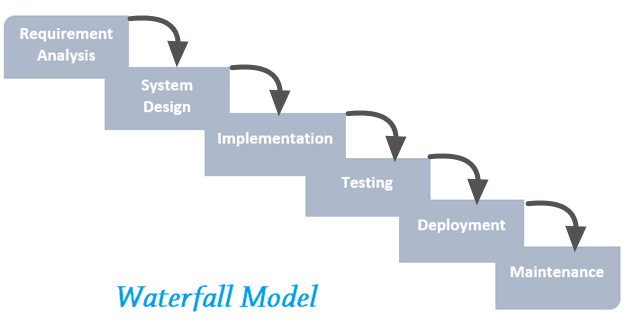
\includegraphics[width=\textwidth]{water}

\end{center}
\caption{Waterfall Model}
\end{figure}


In Waterfall Model phases are executed sequentially, in linear way. We have a steady set of requirements, non changeable in time. The system is developed progressively and the user is involved only in the early phases 
Advantages of this model include it being easy to manage. Disadvantages are that it contains a strict sequence of activities, it has high cost of errors in beginning stages and high importance and cost of documentation and also a contact with the customer is weak. Therefore it can be used when it is possible to precisely define the requirements 

\subsection{Argumentation}

The reasons we have chosen this particular development model are presented below:
\begin{itemize}
\item The sequential order of phases matched perfectly the organized schedule of the development of our Engineering Thesis

\item Fixed set of requirements, as the initial requirements waere submitted by team to the Faculty and could not be changed later
\item Easy management is facilitating our work as we work as a team and have no manager
\item It was highly recommended by the coordinators of the Group Project
\end{itemize}





% ----------------------- Systeem Architecture ------------------


\chapter{System Architecture}



\section{Software Architectural Pattern}


To facilitate the design of classes, we have decided to follow a software architectural pattern. A pattern of choice here was Model–view–controller (MVC) Pattern.
This pattern is used to separate a given application into three interconnected parts. This is done to separate internal representations of information from the ways information is presented to, and accepted from, the user.
\begin{itemize}
\item Model - Model represents an object carrying data. It can also have logic to update controller if its data changes.
\item View - View represents the visualization of the data that model contains.
\item Controller - Controller acts on both model and view. It controls the data flow into model object and updates the view whenever data changes. It keeps view and model separate.
\end{itemize}
\begin{figure}[h!]

\begin{center}

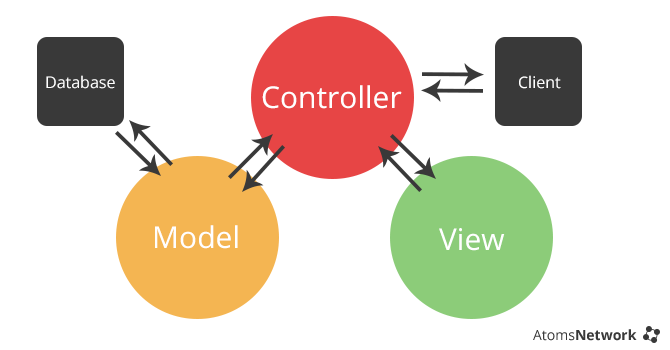
\includegraphics[width=\textwidth]{mvc}

\end{center}
\caption{MVC Pattern}
\end{figure}


As mentioned before, it has helped us develop the division into classes, visible on the class diagram below.
LIME – is the program’s main class.
Then, the Model, View and Controller Classes were designed for each UI element.
The database objects are handled by Servlet (classes taking an article from http POST and passing it to JDBC), DAO (classes responsible for the communication with database) and Query (classes to parse SQL) classes.


\section{Backend Architectural Pattern}

L.I.M.E. project base on many architectural patterns. Precisely chosen patterns make overall architecture strong and well built. 
\subsection{Data Access Object Pattern}

Data access object (DAO) is an object that provides an abstract interface to some type of database or other persistence mechanism. By mapping application calls to the persistence layer, the DAO provides some specific data operations without exposing details of the database. This isolation supports the Single responsibility principle. It separates what data access the application needs, in terms of domain-specific objects and data types (the public interface of the DAO), from how these needs can be satisfied with a specific DBMS, database schema, etc. (the implementation of the DAO).
	The most important fact and advantage is the relatively simple and rigorous separation between two important parts of an application that can but should not know anything of each other, and which can be expected to evolve frequently and independently. Changing business logic can rely on the same DAO interface, while changes to persistence logic do not affect DAO clients as long as the interface remains correctly implemented. All details of storage are hidden from the rest of the application (see information hiding). Thus, possible changes to the persistence mechanism can be implemented by just modifying one DAO implementation while the rest of the application isn't affected.
L.I.M.E. implements one template parent interface with methods which are used by all DAO classes. IBasicCrudRepository extends hibernate CrudRepository and inherits from it all CRUD database operations. Singular DAO classes implement service-specific methods which are defined in DAO interfaces.

\subsection{Plain Old Java Object}

Plain old Java object (POJO) is an ordinary Java object, not bound by any special restriction and not requiring any class path. 
The main aim of the POJO classes is to differentiate business logic from database entity. It makes code cleaner and easier to read and understand.

\begin{figure}[h!]

\begin{center}

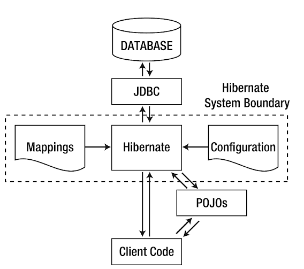
\includegraphics[width=\textwidth]{pojo}

\end{center}
\caption{Plain Old Java Object in Backend Architecture}
\end{figure}
 
The POJO phenomenon has most likely gained widespread acceptance because of the need for a common and easily understood term that contrasts with complicated object frameworks.

L.I.M.E implemens POJO classes for all existing entity class. Those classes are free from frameworks and complicated annotations. There is object mapper implemented, which maps directly Entity to POJO.


\subsection{Dependency Injection}

Dependency Injection is a kind of broader version of "inversion of control" (IoC) principle. It relates to the way in which an object obtains references to its dependencies - the object is passed its dependencies through constructor arguments or after construction through setter methods or interface methods. It is called dependency injection since the dependencies of an object are 'injected' into it, the term dependency is a little misleading here, since it is not a new 'dependency' which is injected but rather a 'provider' of that particular capability. For example, passing a database connection as an argument to a constructor instead of creating one internal would be categorized as dependency injection.
The pattern seeks to establish a level of abstraction via a public interface and to remove dependencies on components by supplying a 'plugin' architecture. This means that the individual components are tied together by the architecture rather than being linked together themselves. The responsibility for object creation and linking is removed from the objects themselves and moved to a factory.


\begin{figure}[h!]

\begin{center}

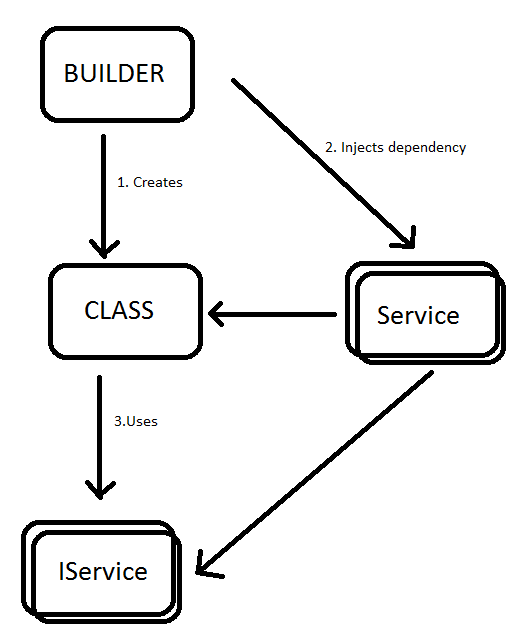
\includegraphics[width=\textwidth]{dependency}

\end{center}
\caption{Dependency Injection}
\end{figure}
 
The main advantage of Dependency Injection is fact that there is only one instance of each object shared through multiple controllers. What is more, it allows a client the flexibility of being configurable. Only the client's behavior is fixed. The client may act on anything that supports the intrinsic interface the client expects.
Dependency injection can be used to externalize a system's configuration details into configuration files, allowing the system to be reconfigured without recompilation. Separate configurations can be written for different situations that require different implementations of components. This includes, but is not limited to, testing.
	L.I.M.E. uses spring dependency injection. There are bean services, which implements the domain logic. Each service implements interface defining the methods. Interfaces and services corresponds to hibernate entities and fulfill the needs of application logic. Interface beans are autowired into the REST controllers.

\subsection{RESTful API}

REpresentational State Transfer (REST) is an architectural style that defines a set of constraints and properties based on HTTP. REST-compliant web services allow the requesting systems to access and manipulate textual representations of web resources by using a uniform and predefined set of stateless operations. Other kinds of web services, such as WSDL and SOAP, expose their own arbitrary sets of operations.
In a RESTful web service, requests made to a resource's URI will elicit a response that may be in XML, HTML, JSON, or some other format. The response may confirm that some alteration has been made to the stored resource, and the response may provide hypertext links to other related resources or collections of resources. When HTTP is used, as is most common, the operations available are GET, POST, PUT, DELETE, and other predefined CRUD HTTP methods. 


\begin{figure}[h!]

\begin{center}

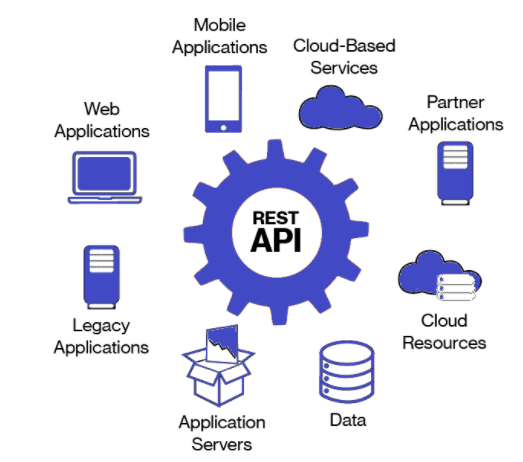
\includegraphics[width=\textwidth]{rest}

\end{center}
\caption{RESTful API}
\end{figure}
 
L.I.M.E. implements RESTful controllers which are used to communicate with a client part of application. It communicates with JSON body type. There are CRUD used methods like PUT, DELETE, POST, GET to make action more readable and indicate what exactly it does. There are Controllers corresponding to view in a client part. .


% ----------------------- Technical Analysis ------------------


\chapter{Technical Analysis}


\section{Client-Server Architecture}

Client/server architecture is a producer/consumer computing architecture where the server acts as the producer and the client as a consumer. The server houses and provides high-end, computing-intensive services to the client on demand.
L.I.M.E. implements client-service architecture. There are 2 applications in the project:
\begin{enumerate}
\item Server implemented in JAVA,
\item GUI implemented with AngularJS
\end{enumerate}
Communication between client and server is done with RESTful API. Server accepts request from authenticated users sent from GUI. Then process it, saves data in database and sends answer.

\begin{figure}[h]

\begin{center}

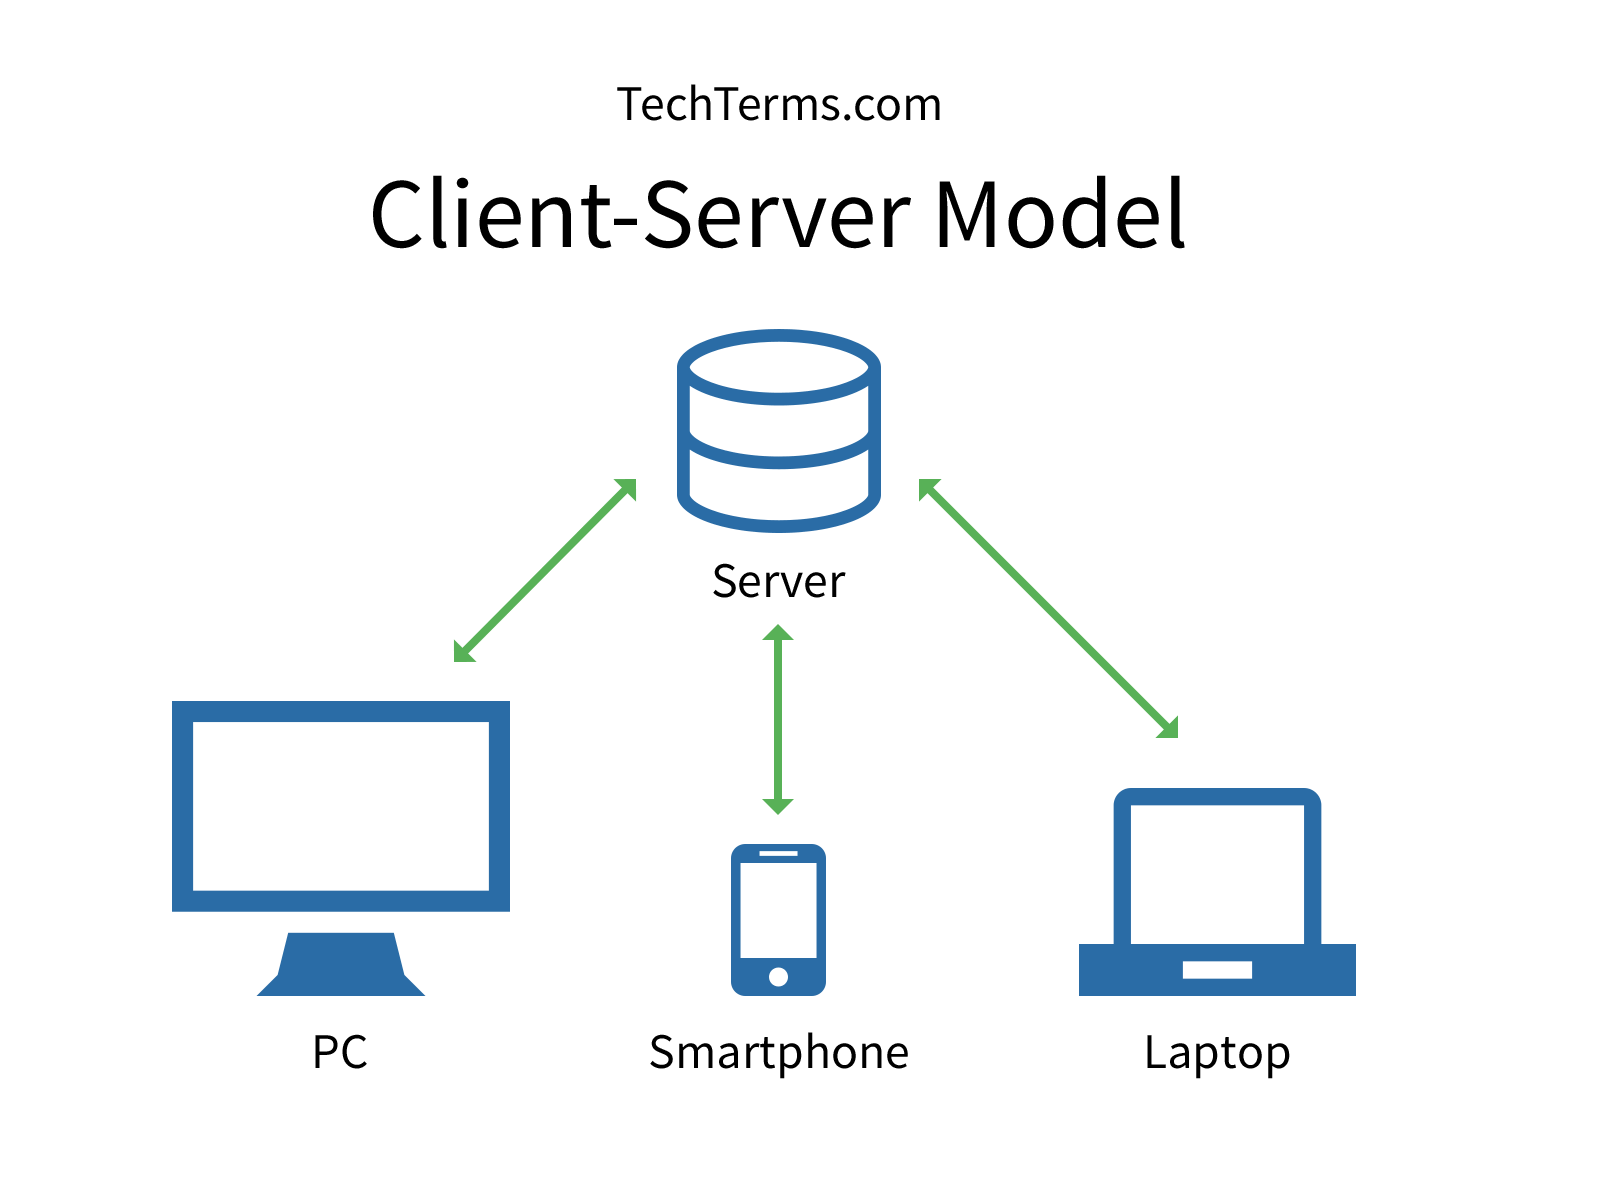
\includegraphics[width=\textwidth]{CS}

\end{center}
\caption{Client-Server Architecture}
\end{figure}

\section{Login}
 L.I.M.E. application have got system to recognize users and its roles. It is implemented using Spring Security. When the user logs in GUI application sends login request to server and the server application checks if the user exist and it’s roles. In the response, it passes the authorization data which is valid for 12 hours (session timeout). Each request from GUI to Server contains a header with the authorization data, so server can recognize which user sends request and if has appropriate roles.
\section{Program Interface}


\section{System Classes}

The Application is composed with the following packages, and the package contain the following classes and interfaces:

\begin{enumerate} 
\item Lime	 
\begin{enumerate} 
\item \textbf{LimeApplication}	The Main Class for Lime Application.
\end{enumerate} 
\item Api	 
\begin{enumerate} 
\item \textbf{GlobalExceptionHandlingControllerAdvice} Performs exception handling for all REST API controller.
\end{enumerate} 
\item ClassModels	 
\begin{enumerate} 
\item \textbf{DrawSeries} The class for Plotting Time Series into a Chart
\item \textbf{TimeSeries} The class of Time Series
\end{enumerate} 
\item Config	 
\begin{enumerate} 
\item \textbf{SecurityConfiguration} The type Security configuration.
\item \textbf{StorageProperties} The type Storage properties.
\item \textbf{SwaggerConfig} Main configuration class to enable the Swagger UI frontend.
\end{enumerate} 
\item Controller	 
\begin{enumerate} 
\item \textbf{BaseController} The Basic type of controller
\item \textbf{DevController} The type Dev controller.
\item \textbf{FileUploadController} The type File upload controller.
\item \textbf{ForecastController} The type Forecast controller.
\item \textbf{FormulaController} The type Formula controller.
\item \textbf{JobController} The type Job controller.
\item \textbf{OrderController} The type Order controller.
\item \textbf{ProductCategoryController} The type Product category controller.
\item \textbf{ProductController} The type Product controller.
\item \textbf{ReportController} The type Report controller.
\item \textbf{ResourceCategoryController} The type Resource category controller.
\item \textbf{ResourceController} The type Resource controller.
\item \textbf{SupplierController} The type Supplier controller.
\item \textbf{UserController} The type User controller.

\end{enumerate} 
\item Dao	 
\begin{enumerate} 
\item \textbf{IBasicCRUDRepository<T,ID extends java.io.Serializable>} The interface Basic crud repository.
\item \textbf{IFormulaDAO} The interface Formula dao.
\item \textbf{IJobDAO} The interface Job dao.
\item \textbf{IProductCategoryDAO} The interface Product category dao.
\item \textbf{IProductDAO} The interface Product dao.
\item \textbf{IResourceCategoryDAO} The interface Resource category dao.
\item \textbf{IResourceDAO} The interface Resource dao.
\item \textbf{IRoleDAO} The interface Role dao.
\item \textbf{ISupplierDAO} The interface Supplier dao.
\item \textbf{IUserDAO} The interface User dao.

\end{enumerate} 
\item Exception	 
\begin{enumerate} 
\item \textbf{AlreadyExistsException} thrown when an entity with at leas one unique field already exists .
\item \textbf{ForbiddenException} thrown when eg. an authentication attempt is not allowed with the given credentials (not details returned).
\item \textbf{IllegalDataException} thrown when the given data is not valid in the current context.
\item \textbf{InvalidRequestException} thrown when a request is invalid in the current context.
\item \textbf{NotAcceptableException} exception, thrown when given data is not acceptable.
\item \textbf{NotFoundException} thrown when an entity is not found where it is expected.
\item \textbf{OperationNotAllowedException} thrown when a contract management API call is not allowed.
\item \textbf{ServiceUnavailableException} The type Service unavailable exception.
\item \textbf{StorageException} The type Storage exception.
\item \textbf{StorageFileNotFoundException} The type Storage file not found exception.
\item \textbf{UnprocessableEntityException} thrown when an entity contains validation errors.

\end{enumerate} 
\item Model	 
\begin{enumerate} 
\item \textbf{CustomUserDetails} The type Custom user details.
\item \textbf{Formula} Model representation of a formula used in Lime.
\item \textbf{Job} Model representation of a job created by Lime user.
\item \textbf{Product} Model representation of a product added in Lime.
\item \textbf{ProductCategory} The type Product category.
\item \textbf{Resource} Model representation of a resource used in Lime.
\item \textbf{ResourceCategory} The type Resource category.
\item \textbf{Role} Model representation of a user role in Lime.
\item \textbf{Supplier} Model representation of a supplier in Lime.
\item \textbf{User} Model representation of user of Lime.

\end{enumerate} 
\item Pojo	 
\begin{enumerate} 
\item \textbf{BasicPOJO} The type Basic pojo.
\item \textbf{FormulaPOJO} The type Formula pojo.
\item \textbf{JobPOJO} The type Job pojo.
\item \textbf{ProductCategoryPOJO} The type Product category pojo.
\item \textbf{ProductPOJO} The type Product pojo.
\item \textbf{ResourceCategoryPOJO} The type Resource category pojo.
\item \textbf{ResourcePOJO} The type Resource pojo.
\item \textbf{RolePOJO} The type Role pojo.
\item \textbf{SupplierPOJO} The type Supplier pojo.
\item \textbf{UserPOJO} The type User pojo.

\end{enumerate} 
\item Service	 
\begin{enumerate} 
\item \textbf{IBasicCRUDService} The interface Basic crud service.
\item \textbf{IForecastService} The interface Forecast service.
\item \textbf{IFormulaService} The interface Formula service.
\item \textbf{IJobService} The interface Job service.
\item \textbf{IMailService} The interface Mail service.
\item \textbf{INotificationService} The interface Notification service.
\item \textbf{IProductCategoryService} The interface Product category service.
\item \textbf{IProductService} The interface Product service.
\item \textbf{IReportService} The interface Report service.
\item \textbf{IResourceCategoryService} The interface Resource category service.
\item \textbf{IResourceService} The interface Resource service.
\item \textbf{IRoleService} The interface Role service.
\item \textbf{ISmoothingService} The interface Smoothing service.
\item \textbf{IStorageService} The interface Storage service.
\item \textbf{ISupplierService} The interface Supplier service.
\item \textbf{ITimeSeriesService} The interface Time series service.
\item \textbf{IUserService} The interface User service.

\end{enumerate} 
\begin{enumerate} 
\item \textbf{BasicCRUDService} The type Basic crud service.
\item \textbf{CustomUserDetailsService} The type Custom user details service.
\item \textbf{ForecastService} The type Forecast service.
\item \textbf{FormulaService} The type Formula service.
\item \textbf{JobService} The type Job service.
\item \textbf{MailService} The type Mail service.
\item \textbf{NotificationService} The type Notification service.
\item \textbf{ProductCategoryService} The type Product category service.
\item \textbf{ProductService} The type Product service.
\item \textbf{ReportService} The type Report service.
\item \textbf{ResourceCategoryService} The type Resource category service.
\item \textbf{ResourceService} The type Resource service.
\item \textbf{RoleService} The type Role service.
\item \textbf{SmoothingService} The type Smoothing service.
\item \textbf{StorageService} The type Storage service.
\item \textbf{SupplierService} The type Supplier service.
\item \textbf{TimeSeriesService} The type Time series service.
\item \textbf{UserService} The type User service.

\end{enumerate} 
\item Tools
\begin{enumerate} 
\item \textbf{DBPopulator} The type Database populator.
\item \textbf{ParseTools} The type Parse tools.
\item \textbf{StartUpPopulator} 
\item \textbf{TSGenerator} The type Time Series generator.

\end{enumerate}
\end{enumerate}

\section{Database Design}

\begin{figure}[hb!]

\begin{center}

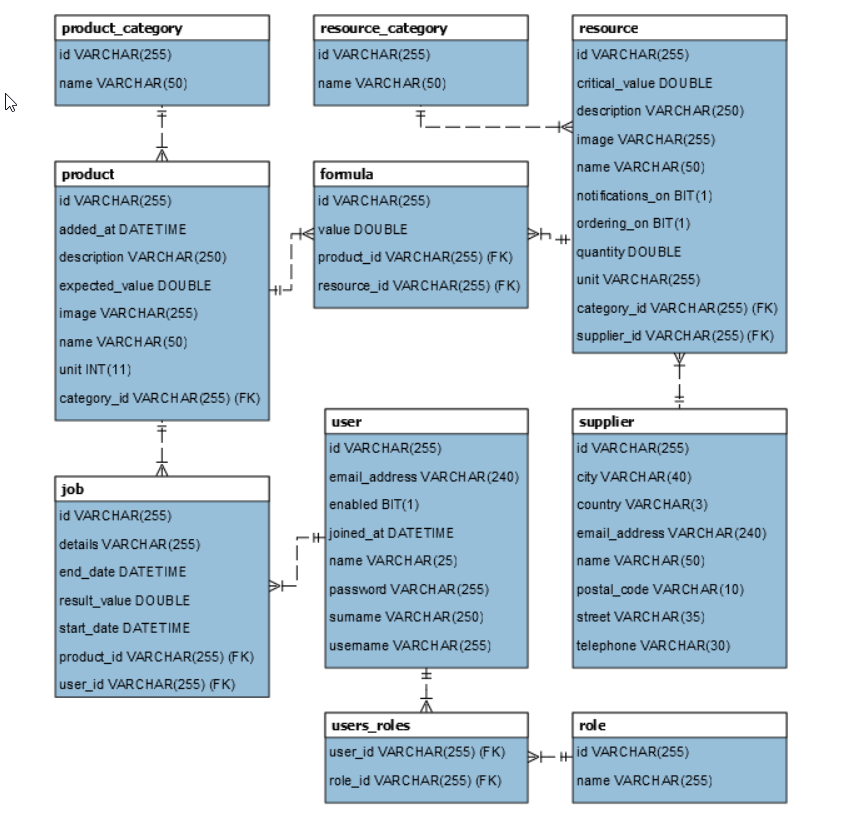
\includegraphics{DB4}

\end{center}
\caption{Database Design}
\end{figure}

The database consists of the following tables:

\begin{enumerate}
\item \textbf{Product} Stores information about products (complex structures of resources) with their properties:
\begin{enumerate}
\item \textbf{Product ID} ID of a product
\item \textbf{Added At} Date of adding a product to a database
\item \textbf{Describtion} Describtion of a product
\item \textbf{Expected Value} Expected value - how much of a product shall be obtained after production
\item \textbf{Image} Image for this product
\item \textbf{Name} Name of a product
\item \textbf{Unit} Unit of a measurement
\item \textbf{Category ID} Assigns a product to a category
\end{enumerate}

\item \textbf{Product Category} Stores information about product categories: its name and ID

\item \textbf{Job} Logs the jobs performed by the user and the following details:
\begin{enumerate}
\item \textbf{Job ID} ID of a job
\item \textbf{Details}More details about the job
\item \textbf{Result Value} Result value - how much of a product was actually obtained after production
\item \textbf{Start Date} Start date of a job
\item \textbf{End Date} End date of a job
\item \textbf{Product ID} ID of a product that resulted from this job
\item \textbf{User ID} Assigns a job to a user which have performed it
\end{enumerate}

\item \textbf{User}  This table stores properties of every user of the system, such as:
\begin{enumerate}
\item \textbf{User ID} ID of a user
\item \textbf{Email address} Email address of this user
\item \textbf{Enabled} Is this an active user of the system
\item \textbf{Joined At} Date of joining the system
\item \textbf{Name} Given Name
\item \textbf{Surname} Surname
\item \textbf{Username} Username chosen by the user
\item \textbf{Password} User's password in encrypted form
\end{enumerate}

\item \textbf{User Roles} Assigns users to their roles (resolves the many-to-many relationship)

\item \textbf{Role} Stores each role with its name and ID

\item \textbf{Formula}  Resolves the many-to-many relation between resources and product, represents the quantity of resources used to make a product
\begin{enumerate}
\item \textbf{Formula ID} ID of a formula
\item \textbf{Product ID} ID of a product
\item \textbf{Resource ID} ID of a resource
\item \textbf{Value} How much of a given resource is neede to make the given product
\end{enumerate}

\item \textbf{Resource}  Stores information about a basic laboratory resource and its properties, such as:
\begin{enumerate}
\item \textbf{Product ID} ID of a resource
\item \textbf{Describtion} Describtion of a resource
\item \textbf{Image} Image for the resource
\item \textbf{Name} Name of a resource
\item \textbf{Critical Value} critical value - how much of a resource shall be left for the notifications of the low level of resource to be triggered
\item \textbf{Notifiactions On} Are the notifications about the low level of the resource turned on
\item \textbf{Ordering On} Is automatic ordering of the resource turned on
\item \textbf{Quantity} How much of a resource at the storage at the moment
\item \textbf{Unit} Unit of a measurement
\item \textbf{Category ID} Assigns a resource to a category
\item \textbf{Supplier ID} Assigns a resource to a supplier
\end{enumerate}

\item \textbf{Resource Category} Stores information about resource categories: its name and ID

\item \textbf{Supplier} Stores data about suppliers assigned to each resources
\begin{enumerate}
\item \textbf{Supplier ID} ID of a supplier
\item \textbf{Email address} Email address of this supplier
\item \textbf{Name} Name of the supplier
\item \textbf{Street} Address of the supplier: street name and number
\item \textbf{City} Address of the supplier: City
\item \textbf{Postal Code} Address of the supplier: Postal Code
\item \textbf{Country} Address of the supplier: Country
\item \textbf{Telephone} Telephone number of this supplier
\end{enumerate}

\end{enumerate}
 
\section{Prediction Model}

The prediction of the future values of production of products and usage of resources is one of the key features of the application.
For the prediction model, many known models for time series prediction were researched, until we found the one that was appropriate to use in the application. The Exponential Smoothing Method was chosen for the following reasons:
\begin{enumerate}
\item The set of variables is rather small and rather simple - no reason to use more sophisticated methods.
\item The prediction model was to be implemented from scratch and Exponential Smoothing. Many more complicated methods could have been imported into the application using libraries, but the decision was that it would be more challenging for the project to take one of the less complicated methods and implement every step of it on our own.
\end{enumerate}

\begin{definition}[Mean Squared Error]
Parę uporządkowaną $(A,F)$, gdzie $A\neq \emptyset$ jest zbiorem, a $F$ jest rodziną operacji określonych na $A$, nazywamy \textit{algebrą} (lub \textit{$F$-algebrą}). Zbiór $A$ nazywa się \textit{zbiorem elementów}, \textit{nośnikiem} lub \textit{uniwersum} algebry $(A,F)$, a $F$ \textit{zbiorem operacji elementarnych}.
\end{definition}
The alpha and beta coefficients used for the calculation of smoothing are being optimized so that the Mean Squared Error is minimized.


% ----------------------- Experimental Evaluation ------------------

\chapter{Post Execution Documentation}

In this section the final application was tested against the set of initial requirements. for every requirement given in Chapter 3, discussed is how the particular requirement is implemented in the application.

\section{Evaluating Functional Requirements}

The following sections will discuss how the functional requirements were implemented, separately for every group of users (Administrator, Mangaer and User)

\subsection{Administrator}

\begin{longtable}{|p{4cm}|p{12cm}|}
\caption[Evaluating Functional Requirements for Administrator]{Evaluating Functional Requirements for Administrator}
\label{Evaluating Functional Requirements for Administrator}
\centering
\tabularnewline

\hline
\texttt{Functional Requirement} & \texttt{Implementation} \\ \hline
Log in to the system and change his & L.I.M.E. application recognize users and its roles. It is implemented using spring security. Password can be changed by administrator of the system. \\ \hline
Create, modify and remove an account in the system, modify its roles & Administrator can create account via manage users view. It is possible to chose within 3 roles: administrator, manager, staff. It is also possible to edit or remove an account in the same subpage \\ \hline
View, create, modify and remove resources and products & Administrator can create products and recources in products view and resources view respectively. It is also possible to modify and remove objects in the same subpage. \\ \hline
View, create, modify and remove groups of resources and products & Administrator can create groups of products and recources choosing products or resources in manage groups respectively. It is also possible to modify and remove objects in the same subpage. \\ \hline
View, create, modify formula of the product & Administrator can create formula for the given product choosing resources and putting the needed value. It is possible creade and modify formula in products view. \\ \hline
Denfine, generate and send a report & Administrator can define and generate raport depending on date range and resources or products. It can be done in reports view, product and resource subpage respectively. \\ \hline
Denfine, generate and send a prediction & Administrator can define and generate prediction depending on date range and respoures or products. It can be done in prediction view, product and resource subpage respectively. \\ \hline
Define notifications, turn notifications on & Administrator can define critical value of the resource in notifications view. It will notify with email that resource exceed critical value. It can be set on/off separately for each object or for all with one button. \\ \hline
Create job, declare time range of the job & Administrator can create job of an product and declare time range within the job was done. It can be done in job view \\ \hline
Order resources, turn on/off automatic ordering & Administrator can order the resources - supplier will be notified with a mail. It is possible to group resources and send one order. It is possible to turn on/off automatic orders - order will perform when the resource exceed critical value. It can be done in manage orders view. \\ \hline


\end{longtable}

\subsection{Manager}

\begin{longtable}{|p{4cm}|p{12cm}|}
\caption[Evaluating Functional Requirements for Manager]{Evaluating Functional Requirements for Manager}
\label{Evaluating Functional Requirements for Manager}
\centering
\tabularnewline

\hline
\texttt{Functional Requirement} & \texttt{Implementation} \\ \hline

Log in to the system & L.I.M.E. application recognize users and its roles. It is implemented using spring security. Password can be changed by administrator of the system. \\ \hline
View, create, modify and remove resources and products & Manager can create products and recources in products view and  resources view respectively. It is also possible to modify and remove objects in the same subpage. \\ \hline
Define, generate and send a report & Manager can define and generate raport depending on date range and resoures or products. It can be done in reports view, product and resource subpage respectively. \\ \hline
Define, generate and send a prediction & Manager can define and generate prediction depending on date range and resoures or products. It can be done in prediction view, product and resource subpage respectively. \\ \hline
Define notifications, turn notifications on & Manager can define critical value of the resource in notifications view. It will notify with email that resource exceed critical value. It can be set on/off separately for each object or for all with one button. \\ \hline
Order resources, turn on/off automatic ordering & Manager can order the resources - supplier will be notified with a mail. It is possible to group resources and send one order. It is possible to turn on/off automatic orders - order will perform when the resource exceed critical value. It can be done in manage orders view. \\ \hline
Create job, declare time range of the job & Manager can create job of an product and declare time range within the job was done. It can be done in job view. \\ \hline



\end{longtable}

\subsection{User}

\begin{longtable}{|p{4cm}|p{12cm}|}
\caption[Evaluating Functional Requirements for User]{Evaluating Functional Requirements for User}
\label{Evaluating Functional Requirements for User}
\centering
\tabularnewline

\hline
\texttt{Functional Requirement} & \texttt{Implementation} \\ \hline
Log in to the system & L.I.M.E. application recognize users and its roles. It is implemented using spring security. Password can be changed by administrator of the system. \\ \hline
Create job, declare time range of the job & User can create job of an product and declare time range within the job was done. It can be done in job view. \\ \hline


\end{longtable}

\section{Evaluating Non-Functional Requirements}

Similarly, this section will discuss how the non-functional requirements were implemented

\begin{longtable}{|p{3cm}|p{7cm}|p{6cm}|}
\caption[Evaluating Non-Functional Requirements]{Evaluating Non-Functional Requirements}
\label{Evaluating Non-Functional Requirements}
\centering
\tabularnewline

\hline
\texttt{Area} & \texttt{Non-Functional Requirement} & \texttt{Implementation} \\ \hline
Usability & Application must be responsive. It must be working on PC, tablets
and phones with resolution at least 720p. & GUI is implemented with responsive frameworks: Angular and bootstrap \\ \hline
Reliability & Application must be of type High Availability. It should be available
24h/7d between 08:00 and 23:00. There could be service
breaks during the week between 24:00 and 8:00. & Application is deployed on heroku. It uses database mysql addon. It runs 24/7 \\ \cline{2-3}
 & Application must have quick restart in case of app machine failures. & It is possible to restart app with command: heroku restart \\ \hline
Recovery & Application must have daily database backup performed  24:00 and 08:00. & 
Database has default scheduled database dumps. It can be resheduled in heroku db configuration \\ \hline
Performance & Application should respond no longer than 3 seconds while strain
being on level 100 queries per minute. & Application uses client server architecture. RESTful api deliver much higher capacity. \\ \hline
Supportability & Documentation should contain instruction for recovery data from
database backup. & There is delivered step by step manual with database backup manual and sheduled and recovery. \\ \cline{2-3}
 & Application should keep backward compatibility between the released
versions. & With the future releases version, there will be database script provided, which will fill previous entries. \\ \hline
Security & Application must have user levels security. It shall not pass a user who has inappropriate privileges. & Application has implemented user service implemented with spring security, which validates if the user exists and check for each REST endpoint if the user has appropriate privileges. \\ \hline

\end{longtable}



% ----------------------- Conclusions ------------------
\chapter*{Conclusions}

One of the most important goal of our thesis was to deliver a software that will be used by the consumer of the market. Work began with market research. We received several proposals and chose the one that we considered the most appropriate. We decided to develop the ultimate system to manage the warehouse and human resources of the laboratory. Our project – L.I.M.E (Laboratory Internal Management Entity) was developed in line with market needs, consulted with major consumers.\\ \\
At first, we had to decide how the database will look like - what entities, relations, type of the database. That is the fundamental part of the application. We can say with pride, that we achieved excellent  result. There were only few minor changes, most of the primal database project fulfilled needs of the application.\\ \\
Secondly, we had to develop basic back-end parts of the application. Connection with database, user authentication and roles. Many helpers like database populator for test purposes.  \\ \\
Subsequently we had to start develop the client application. This was the hardest part of the work. It was hard to write simultaneously front-end and back-end. There was many  disagreements, and we had to discuss for a long time often to come to the best solutions.\\ \\
Afterwards, when we had already most of the functionalities, we started to develop features that uses most of the functionalities – reports, predictions, notifications. It required knowledge from the area of algorithms and mathematics. \\ \\
To develop our application, we used the top software technologies. Server side is built with Java, Spring, SpringBoot, SpringSecurity, MySQL and the client with AngularJS, Bootstrap. The communication between units is made with RESTful API. The we well-known and wide used solutions helped us to achieve success. \\ \\
During all the time we were documenting each progress we made. The documentation is essential for our project. We need to deliver all manuals and support for the consumers, to help them understand how to properly use and take full advantage of L.I.M.E. \\ \\
Despite the many difficulties we encountered and the fact that it took about 40\% more time than we expected, we are happy, because there are some people, who will use. We have meet our goals and we can say with pride that we achieved great success!

\thispagestyle{empty}




% ------------------------------- BIBLIOGRAPHY ---------------------------
% LEXICOGRAPHICAL ORDER BY AUTHORS' LAST NAMES
% FOR AMBITIOUS ONES - USE BIBTEX


\begin{thebibliography}{20} % IF YOU HAVE MORE REFERENCES, WRITE THE BIGGER NUMBER

\bibitem[1]{Ktos} A. Author, \emph{Title of a book}, Publisher, year, page--page.
\bibitem[2]{Innyktos} J. Bobkowski, S. Dobkowski, Title of an article, \emph{Magazine X, No. 7}, year, PAGE--PAGE.
\bibitem[3]{B} C. Brink, Power structures, \emph{Algebra Universalis 30(2)}, 1993, 177--216.
\bibitem[4]{H} F. Burris, H. P. Sankappanavar, \emph{A Course of Universal Algebra}, Springer-Verlag, New York, 1981.
\end{thebibliography}
\pagenumbering{gobble}
\thispagestyle{empty}



% ----------------------- GLOSSARY ------------------
\chapter*{Glossary}
\begin{longtable}{p{4cm} p{11cm}}


\textbf{Administrator} & A person who is responsible for the upkeep, configuration, and reliable operation of a system.\\ \\
\textbf{Algorithm} & A procedure or formula for solving a problem, based on conductiong a sequence of specified actions. A computer program can be viewed as an elaborate algorithm. \\ \\
\textbf{Angularjs} & A structural framework for dynamic web apps. It lets you use HTML as your template language and lets you extend HTML's syntax to express your application's components clearly and succinctly. \\ \\
\textbf{Application} & A program designed to perform a specific function directly for the user.\\ \\
\textbf{Application Service} & A services that are made available from a business's Web server for Web users or other Web-connected programs. \\ \\
\textbf{Asynchronous} & An adjective describing objects or events that are not coordinated in time.\\ \\
\textbf{Authorization} & The process of giving someone permission to do or have something. In multi-user computer systems, a system administrator defines for the system which users are allowed access to the system and what privileges of use (such as access to which file directories, hours of access, amount of allocated storage space, and so forth). \\ \\
\textbf{Back-End} & Application serves indirectly in support of the front-end services.\\ \\
\textbf{Backup} & Copying of physical or virtual files or databases to a secondary site for preservation in case of equipment failure or other catastrophe. \\ \\
\textbf{Boilerplate} & A unit of writing that can be reused over and over without change. By extension, the idea is sometimes applied to reusable programming as in "boilerplate code."\\ \\
\textbf{Bootstrap} & A free and open-source front-end library for designing websites and web applications. It contains HTML- and CSS-based design templates for typography, forms, buttons, navigation and other interface components, as well as optional JavaScript extensions. \\ \\
\textbf{Browser} & An application program that provides a way to look at and interact with all the information on the World Wide Web. The word "browser" seems to have originated prior to the Web as a generic term for user interfaces that let you browse (navigate through and read) text files online.\\ \\
\textbf{Cloud} & A host on virtual server.\\ \\
\textbf{Cloud-Based} & A software program where cloud-based and local components work together.\\ \\
\textbf{Commit} & The final step in the successful completion of a previously started transaction in a computing system.\\ \\
\textbf{Continuous Deployment} & A strategy for software releases wherein any code commit that passes the automated testing phase is automatically released into the production environment, making changes that are visible to the software's users.\\ \\
\textbf{Dao (Data Access Objects)} & An API that lets a programmer request access to an database.\\ \\
\textbf{Data} & The information that has been translated into a form that is more convenient to move or process.\\ \\
\textbf{Data Availability} & An assurance that data continues to be available at a required level of performance in any situation.\\ \\
\textbf{Database} & A collection of data that is organized so that its contents can easily be accessed, managed, and updated.\\ \\
\textbf{Deploy} & To spread out or arrange strategically.\\ \\
\textbf{Deprecated} & Something is acknowledged but discouraged.\\ \\
\textbf{Development} & The process of conceiving, specifying, designing, programming, documenting, testing, and bug fixing involved in creating and maintaining applications, frameworks, or other software components. \\ \\
\textbf{Distribution} & The phase that follows packaging.\\ \\
\textbf{Endpoint} & Defines the address for a resource , an endpoint is any user device connected to a network.\\ \\
\textbf{Event} & Any identifiable occurrence that has significance for system hardware or software. User-generated events include keystrokes and mouse clicks, among a wide variety of other possibilities.\\ \\
\textbf{Feature} & A distinguishing characteristic of a software item (e.g., performance, portability, or functionality)\\ \\
\textbf{Field} & A location for a single piece of data in a database.\\ \\
\textbf{Foreign Key} & A key that targets a primary key in another table.\\ \\
\textbf{Framework} & A real or conceptual structure intended to serve as a support or guide for the building of something that expands the structure into something useful.\\ \\
\textbf{Front-End} & An application that interacti with users directly.\\ \\
\textbf{Gui} & A graphical user interface to a computer.\\ \\
\textbf{Header} & Something that goes in front of something else and is usually repeated as a standard part of the units of something else\\ \\
\textbf{Heroku} & A cloud-based development platform as a service (PaaS) provider.\\ \\
\textbf{Hosting} & The business of housing, serving, and maintaining files for one or more Web sites. More important than the computer space that is provided for Web site files is the fast connection to the Internet. \\ \\
\textbf{Html (Hypertext Markup Language)} & A standard programming language for describing the contents and appearance of Web pages.\\ \\
\textbf{Insatnce} & In object-oriented programming (OOP), is a specific realization of any object. An object may be varied in a number of ways. Each realized variation of that object is an instance. The creation of a realized instance is called instantiation.\\ \\
\textbf{Integration} & The act of bringing together smaller components into a single system that functions as one.\\ \\
\textbf{Interface} & A group of related methods with empty bodies. Implementing an interface allows a class to become more formal about the behavior it promises to provide. Interfaces form a contract between the class and the outside world, and this contract is enforced at build time by the compiler.\\ \\
\textbf{Iterative} & Used to describe a situation in which a sequence of instructions can be executed multiple times. One pass through the sequence is called an iteration. If the sequence of instructions is executed repeatedly, it is called a loop, and we say that the computer iterates through the loop.\\ \\
\textbf{Jar (Java Archive) } & A package file format typically used to aggregate many Java class files and associated metadata and resources (text, images, etc.) into one file for distribution. \\ \\
\textbf{Java} & Aidely used programming language expressly designed for use in the distributed environment of the internet.\\ \\
\textbf{Javascript} & An interpreted programming or script language from Netscape.\\ \\
\textbf{Json (Javascript Object Notation)} & Text-based, human-readable data interchange format used for representing simple data structures and objects in Web browser-based code.\\ \\
\textbf{Junit} & An open source framework designed for the purpose of writing and running tests in the Java programming language.\\ \\

\textbf{LIME} & Laboratory Internal Management Entity - the name of the application discussed in this document. LIME is the system for resources management in a small chemical laboratory. \\ \\

\textbf{Linux} & An open-source operating system modelled on UNIX.\\ \\
\textbf{Login} & A string used to differentiate between users.\\ \\
\textbf{Manager} & A person who is responsible for the managing resources, products and reports\\ \\
\textbf{Mysql} & An open source relational database management system that uses SQL.\\ \\
\textbf{Password} & A string that authorize access for a gine user login.\\ \\
\textbf{Plugin} & A program that can easily be installed and used as part of another program.\\ \\
\textbf{Primary Key} & A key in a relational database that is unique for each record, used to identify a particular record.\\ \\
\textbf{Query} & A request to a database for information, or to update, modify, or delete information.\\ \\
\textbf{Relational Database} & A collection of data items organized as a set of formally-described tables from which data can be accessed or reassembled in many different ways without having to reorganize the database tables.\\ \\
\textbf{Rest (Representational State Transfer)} & Simple stateless architecture that generally runs over HTTP. It is used to communicate between applications.\\ \\
\textbf{Rollback} & The undoing of partly completed database changes when a database transaction is determined to have failed.\\ \\
\textbf{Row} & A group of fields in a database table organized to contain all the information relevant to a specific entity.\\ \\
\textbf{Server} & A computer program that provides a service to another computer programs (and its user). In the client/server programming model, a server program awaits and fulfills requests from client programs, which may be running in the same or other computers.\\ \\
\textbf{Software} & General term for the various kinds of programs used to operate computers and related devices.\\ \\
\textbf{Spring Framework} & a Injection dependency framework at first (it's still as it is today) targeting managing life-cycle of Java components (what so-called beans). \\ \\
\textbf{Springboot} & A suite, pre-configured, pre-sugared set of frameworks/technologies to reduce boiler plate configuration providing you the shortest way to have a Spring web application up and running with smallest line of code/configuration out-of-the-box. \\ \\
\textbf{Spring security} & A Java/Java EE framework that provides authentication, authorization and other security features for enterprise applications.\\ \\
\textbf{Sql (Structured Query Language)} & A standard interactive and programming language for getting information from and updating a database.\\ \\
\textbf{Staff} & A person who is responsible for endpoint work and jobs.\\ \\
\textbf{Synchronous} & An adjective describing objects or events that are coordinated in time.\\ \\
\textbf{Table} & In a relational database, a data structure that organizes the information about a single topic into rows and columns.\\ \\
\textbf{Upgrade} & A new version of or addition to a hardware or, more often, software product that is already installed or in use.\\ \\
\textbf{Validation} & A quality assurance used to check if the typed data is correct.\\ \\
\textbf{Virtual Server} & A server (computer and various server programs) at someone else's location that is shared by multiple Web site owners so that each owner can use and administer it as though they had complete control of the server.\\ \\
\textbf{War } & A file used to distribute a collection of JAR-files, JavaServer Pages, Java Servlets, Java classes, XML files, tag libraries, static web pages (HTML and related files) and other resources that together constitute a web application. \\ \\
\textbf{Web Application (Web App)} & An application program that is stored on a remote server and delivered over the Internet through a browser interface.\\ \\


\end{longtable}

\thispagestyle{empty}


% ----------------------------  LIST OF FIGURES --------------------------------
\listoffigures
\thispagestyle{empty}
If you don't need it, delete it.


% -----------------------------  LIST OF TABLES --------------------------------
\renewcommand{\listtablename}{List of tables}
\listoftables
\thispagestyle{empty}
If you don't need it, delete it.

% -----------------------------  LIST OF APPENDICES ---------------------------
\chapter*{List of appendices}
\begin{enumerate}
\item Appendix A. User Manual
\item Appendix B. Testing Scenarios
\end{enumerate}
\thispagestyle{empty}


% -----------------------------  APPENDIX A ---------------------------
\chapter*{A. User Manual}

\begin{figure}[h!]
\begin{center}
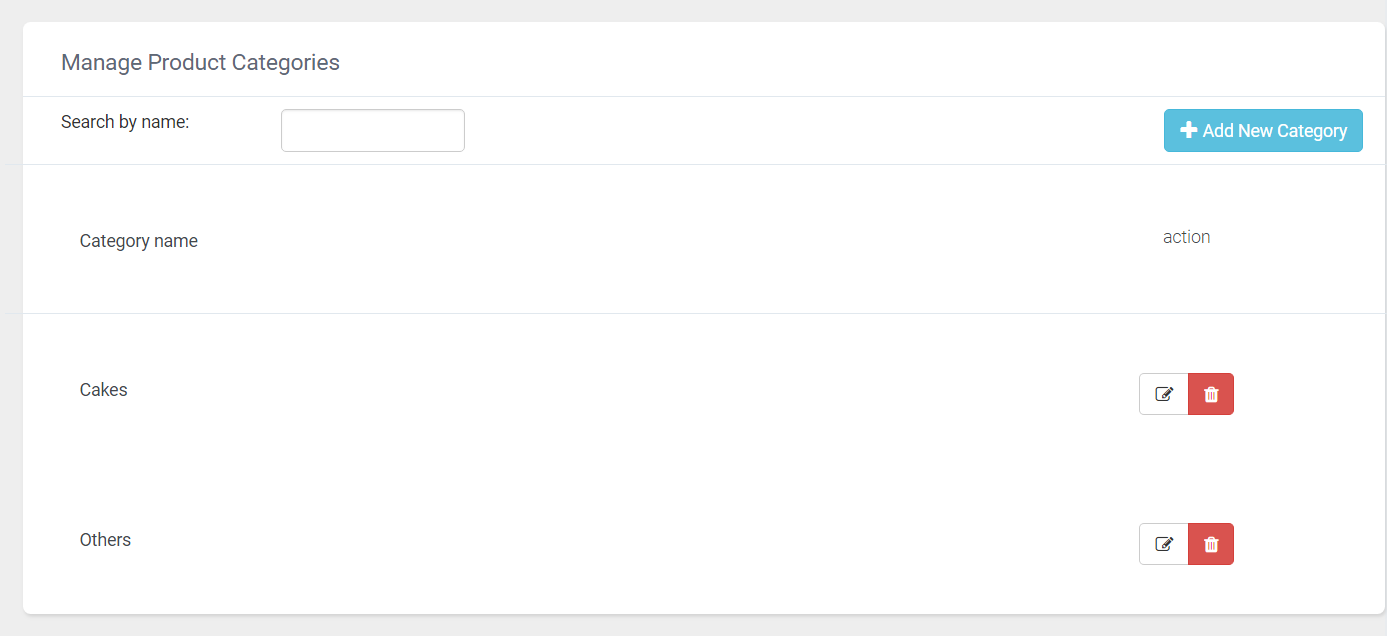
\includegraphics[width=\textwidth]{AS/categories/product/1}
\end{center}
\caption{job1}
\end{figure}

\begin{figure}[h!]
\begin{center}
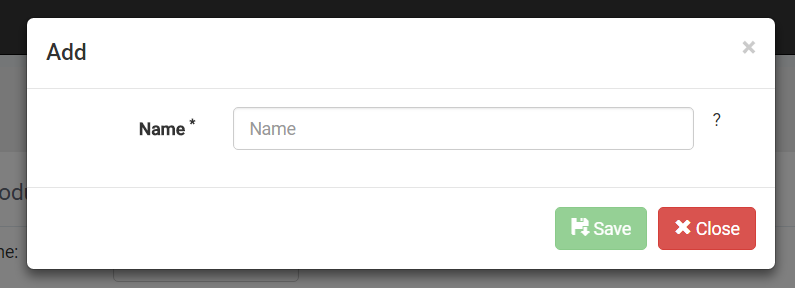
\includegraphics[width=\textwidth]{AS/categories/product/2}
\end{center}
\caption{job1}
\end{figure}

\begin{figure}[h!]
\begin{center}
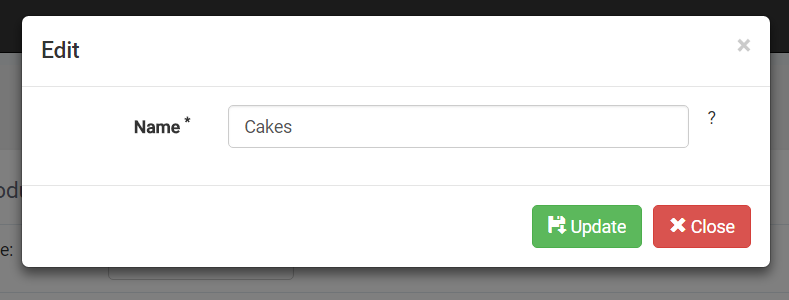
\includegraphics[width=\textwidth]{AS/categories/product/3}
\end{center}
\caption{job1}
\end{figure}

\begin{figure}[h!]
\begin{center}
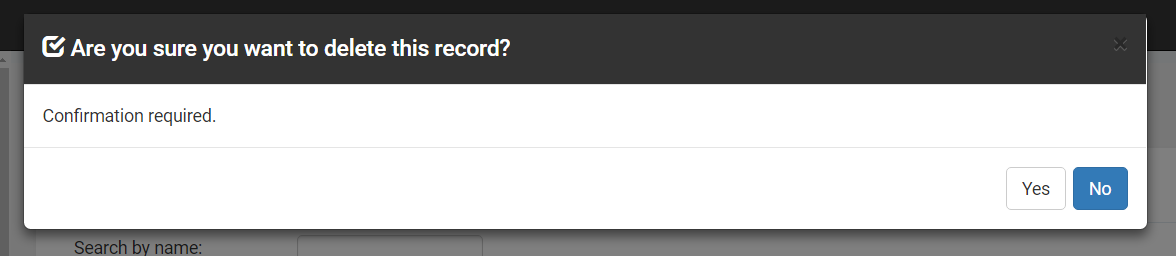
\includegraphics[width=\textwidth]{AS/categories/product/4}
\end{center}
\caption{job1}
\end{figure}


\begin{figure}[h!]
\begin{center}
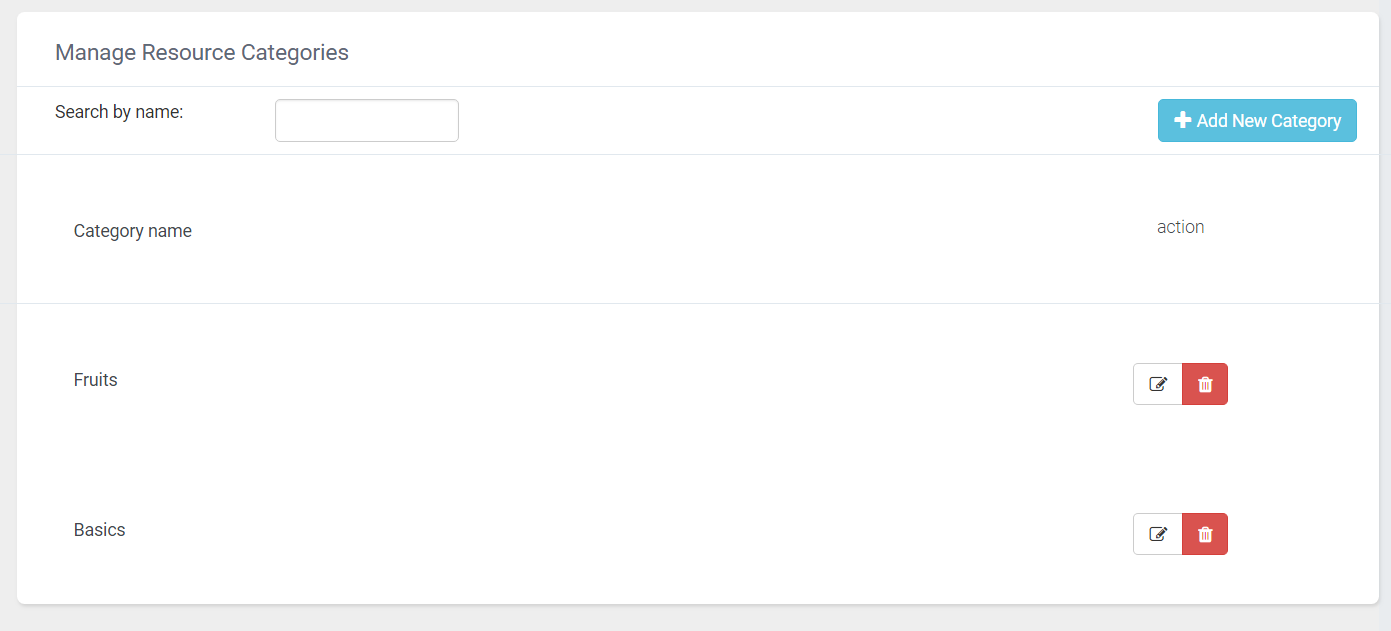
\includegraphics[width=\textwidth]{AS/categories/resource/1}
\end{center}
\caption{job1}
\end{figure}

\begin{figure}[h!]
\begin{center}
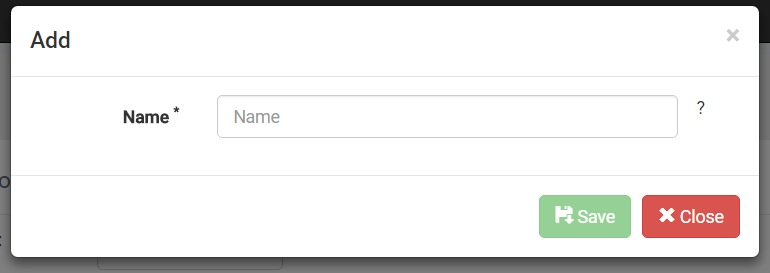
\includegraphics[width=\textwidth]{AS/categories/resource/2}
\end{center}
\caption{job1}
\end{figure}

\begin{figure}[h!]
\begin{center}
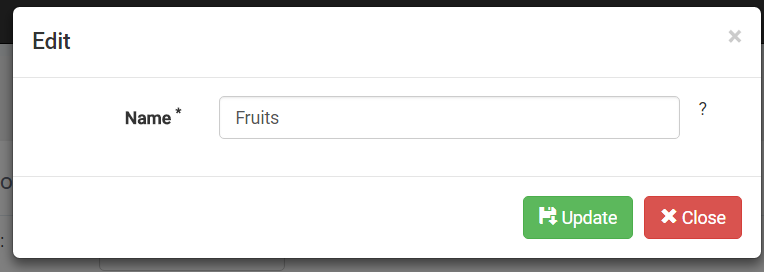
\includegraphics[width=\textwidth]{AS/categories/resource/3}
\end{center}
\caption{job1}
\end{figure}

\begin{figure}[h!]
\begin{center}
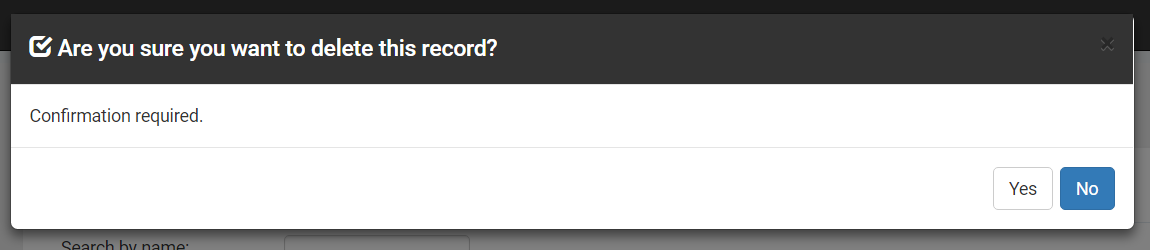
\includegraphics[width=\textwidth]{AS/categories/resource/4}
\end{center}
\caption{job1}
\end{figure}

\begin{figure}[h!]
\begin{center}
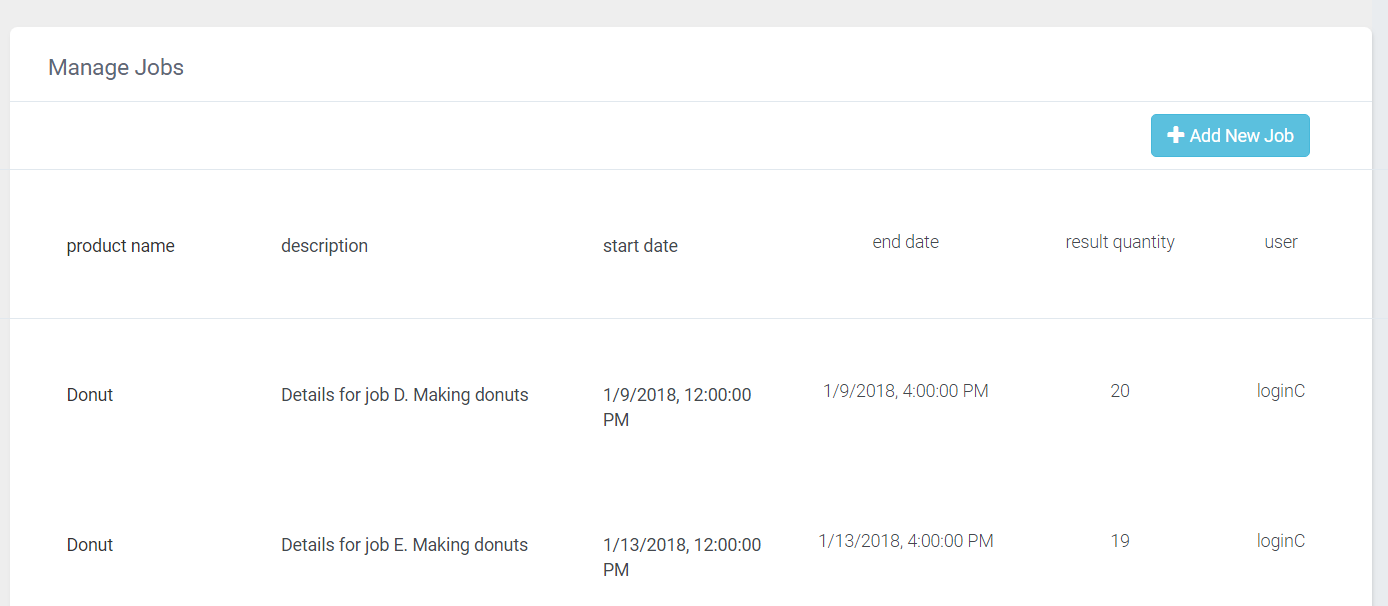
\includegraphics[width=\textwidth]{AS/jobs/1}
\end{center}
\caption{job1}
\end{figure}

\begin{figure}[h!]
\begin{center}
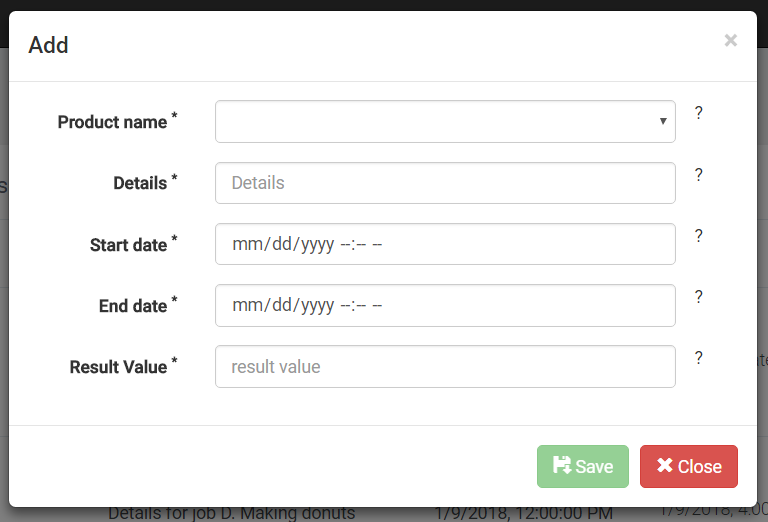
\includegraphics[width=\textwidth]{AS/jobs/2}
\end{center}
\caption{job1}
\end{figure}
\thispagestyle{empty}


\begin{figure}[h!]
\begin{center}
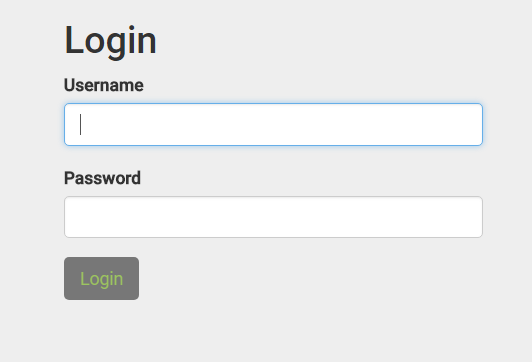
\includegraphics[width=\textwidth]{AS/login/1}
\end{center}
\caption{job1}
\end{figure}

\begin{figure}[h!]
\begin{center}
\includegraphics[width=\textwidth]{AS/login/2}
\end{center}
\caption{job1}
\end{figure}

\begin{figure}[h!]
\begin{center}
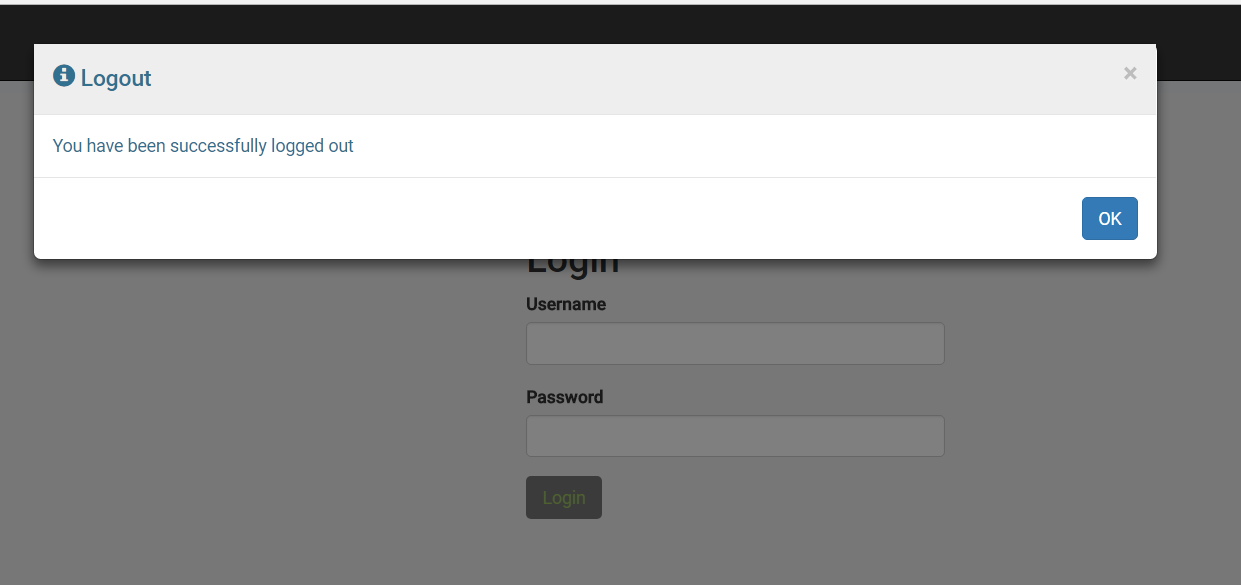
\includegraphics[width=\textwidth]{AS/login/3}
\end{center}
\caption{job1}
\end{figure}

\begin{figure}[h!]
\begin{center}
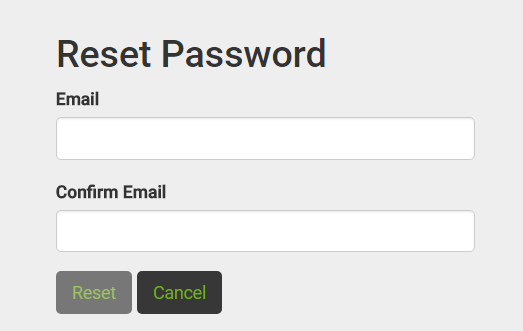
\includegraphics[width=\textwidth]{AS/login/4}
\end{center}
\caption{job1}
\end{figure}

\begin{figure}[h!]
\begin{center}
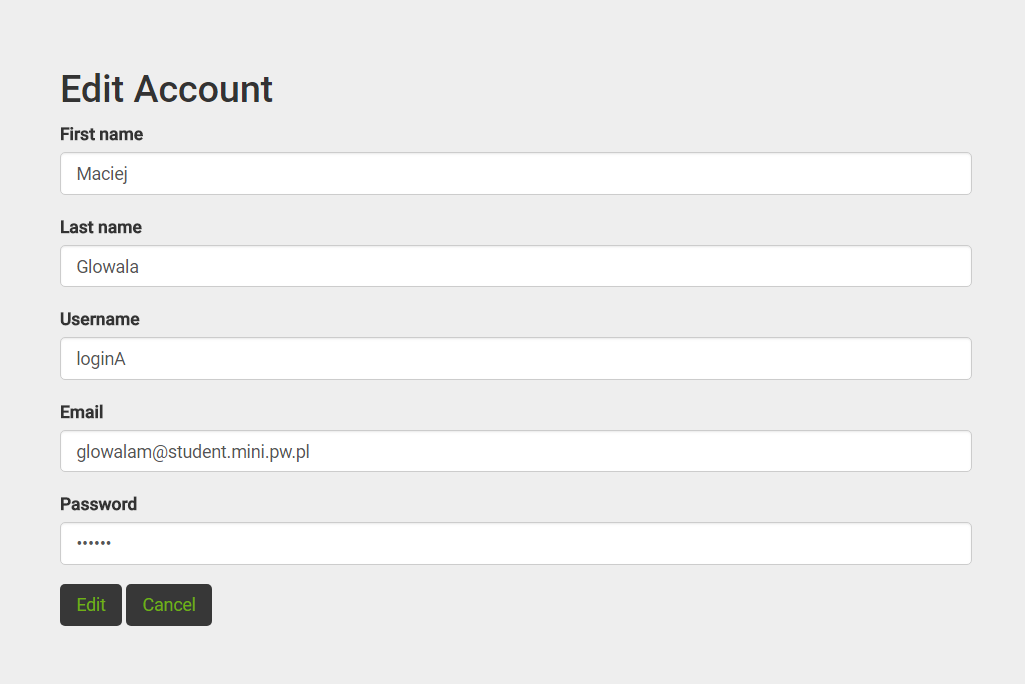
\includegraphics[width=\textwidth]{AS/login/5}
\end{center}
\caption{job1}
\end{figure}

\begin{figure}[h!]
\begin{center}
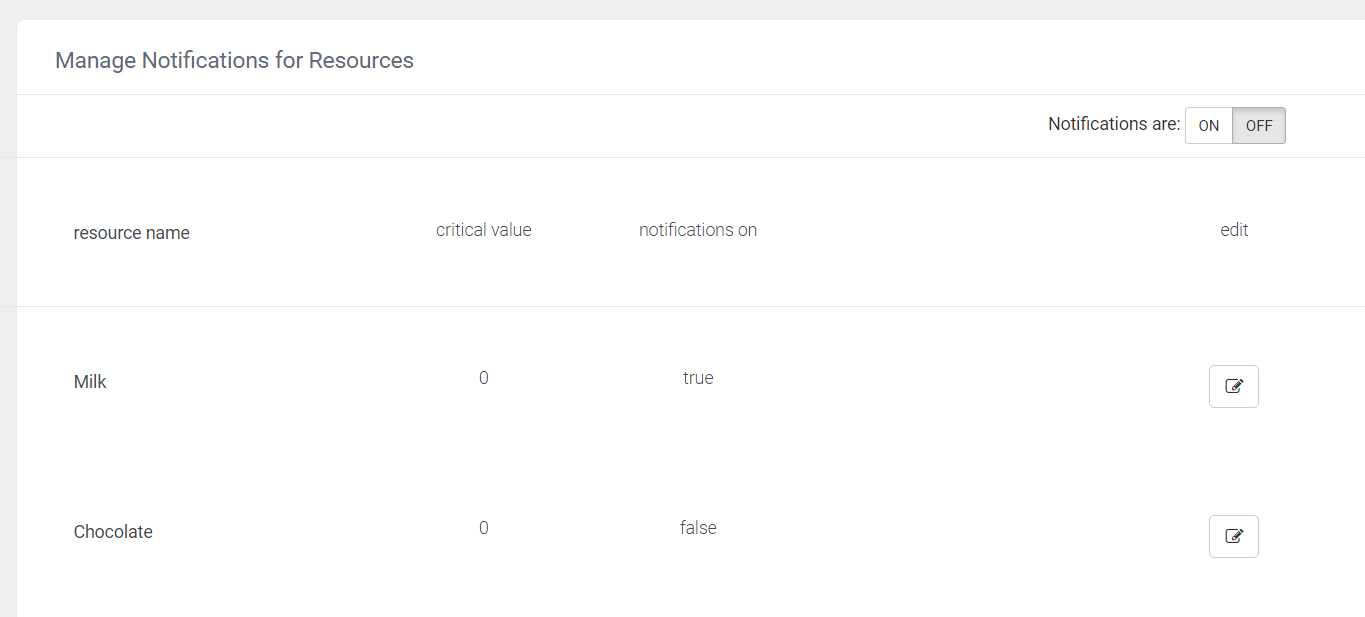
\includegraphics[width=\textwidth]{AS/notifications/1}
\end{center}
\caption{job1}
\end{figure}

\begin{figure}[h!]
\begin{center}
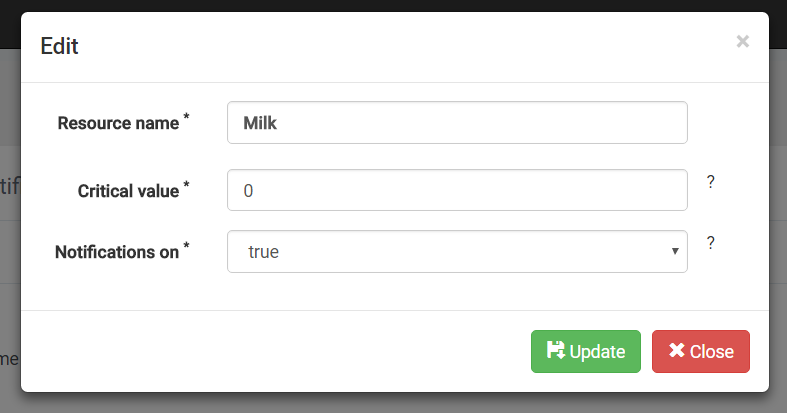
\includegraphics[width=\textwidth]{AS/notifications/2}
\end{center}
\caption{job1}
\end{figure}
\thispagestyle{empty}

\begin{figure}[h!]
\begin{center}
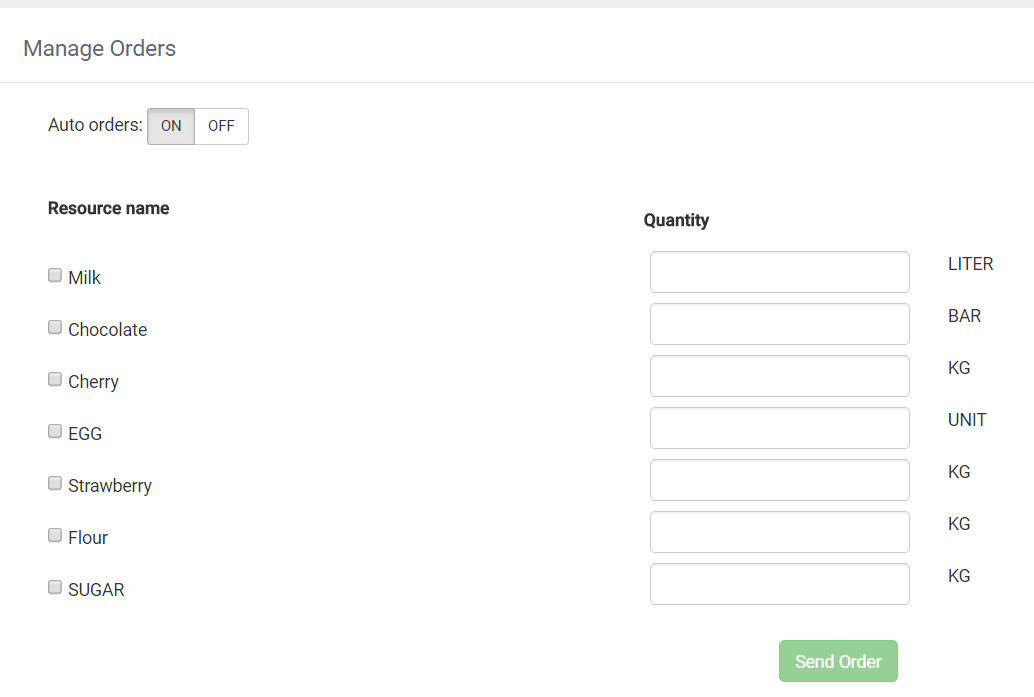
\includegraphics[width=\textwidth]{AS/orders/1}
\end{center}
\caption{job1}
\end{figure}
\thispagestyle{empty}

\begin{figure}[h!]
\begin{center}
\includegraphics[width=\textwidth]{AS/product/1}
\end{center}
\caption{job1}
\end{figure}
\thispagestyle{empty}


\begin{figure}[h!]
\begin{center}
\includegraphics[width=\textwidth]{AS/product/2}
\end{center}
\caption{job1}
\end{figure}
\thispagestyle{empty}


\begin{figure}[h!]
\begin{center}
\includegraphics[width=\textwidth]{AS/product/3}
\end{center}
\caption{job1}
\end{figure}
\thispagestyle{empty}

\begin{figure}[h!]
\begin{center}
\includegraphics[width=\textwidth]{AS/product/4}
\end{center}
\caption{job1}
\end{figure}
\thispagestyle{empty}


\begin{figure}[h!]
\begin{center}
\includegraphics[width=\textwidth]{AS/product/5}
\end{center}
\caption{job1}
\end{figure}
\thispagestyle{empty}


\begin{figure}[h!]
\begin{center}
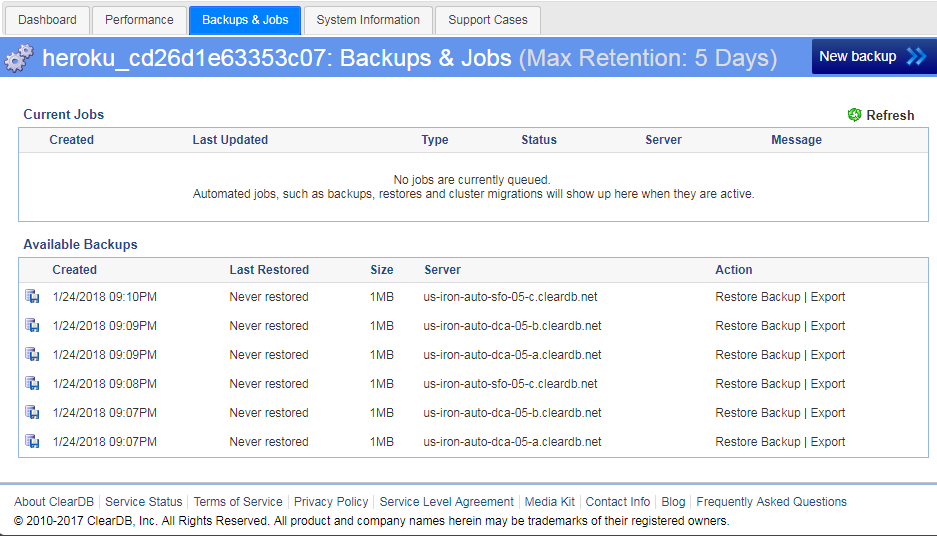
\includegraphics[width=\textwidth]{AS/product/6}
\end{center}
\caption{job1}
\end{figure}
\thispagestyle{empty}

\begin{figure}[h!]
\begin{center}
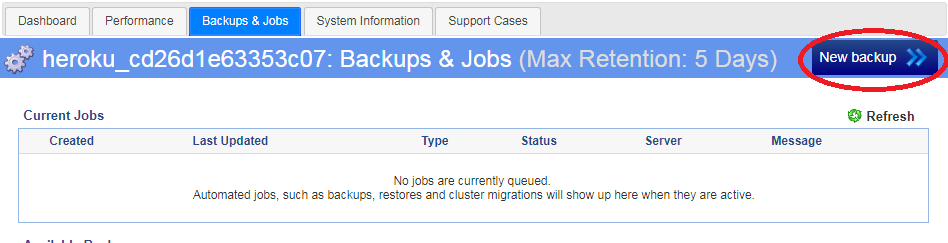
\includegraphics[width=\textwidth]{AS/product/7}
\end{center}
\caption{job1}
\end{figure}
\thispagestyle{empty}

\begin{figure}[h!]
\begin{center}
\includegraphics[width=\textwidth]{AS/resources/1}
\end{center}
\caption{job1}
\end{figure}
\thispagestyle{empty}


\begin{figure}[h!]
\begin{center}
\includegraphics[width=\textwidth]{AS/resources/2}
\end{center}
\caption{job1}
\end{figure}
\thispagestyle{empty}


\begin{figure}[h!]
\begin{center}
\includegraphics[width=\textwidth]{AS/resources/3}
\end{center}
\caption{job1}
\end{figure}
\thispagestyle{empty}

\begin{figure}[h!]
\begin{center}
\includegraphics[width=\textwidth]{AS/resources/4}
\end{center}
\caption{job1}
\end{figure}
\thispagestyle{empty}


\begin{figure}[h!]
\begin{center}
\includegraphics[width=\textwidth]{AS/resources/5}
\end{center}
\caption{job1}
\end{figure}
\thispagestyle{empty}


\begin{figure}[h!]
\begin{center}
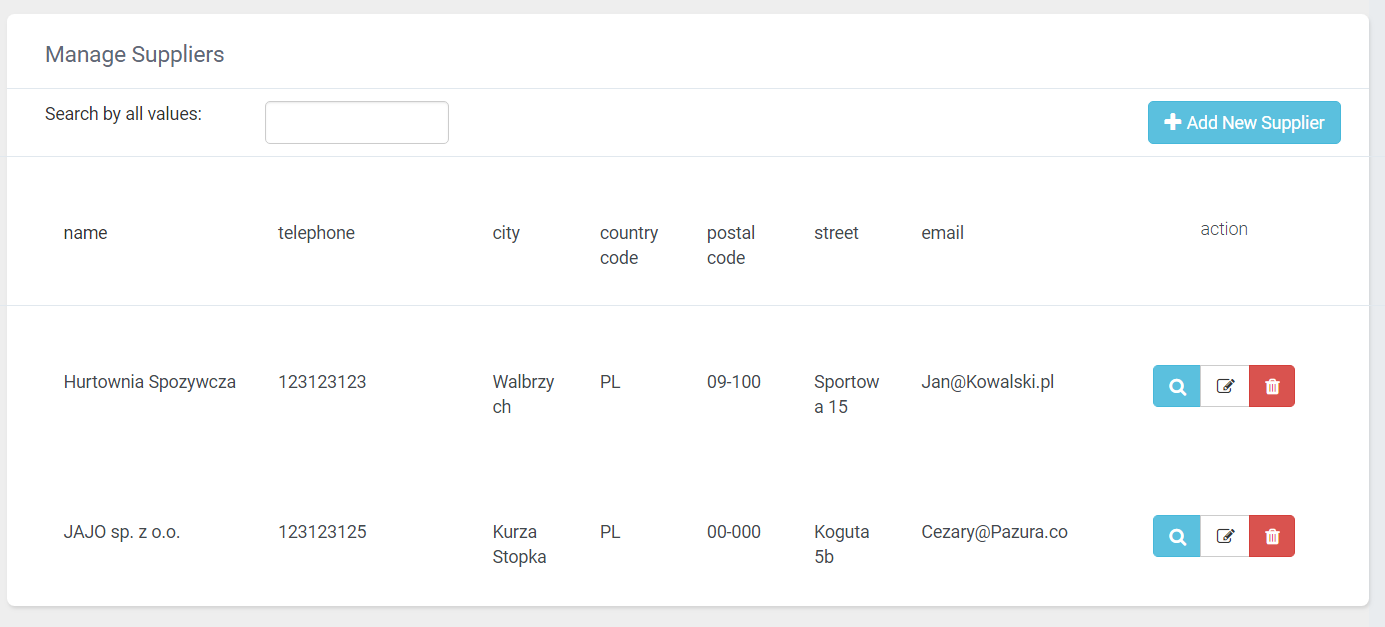
\includegraphics[width=\textwidth]{AS/supplier/1}
\end{center}
\caption{job1}
\end{figure}
\thispagestyle{empty}


\begin{figure}[h!]
\begin{center}
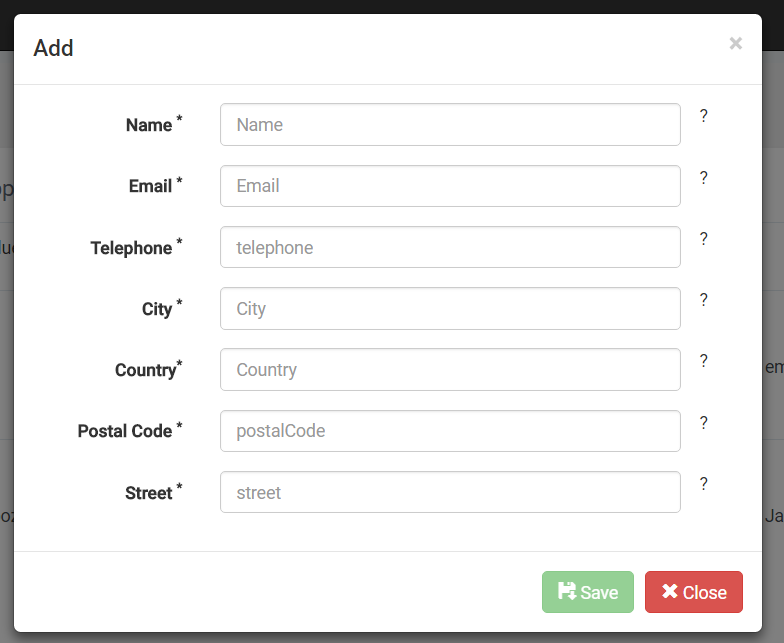
\includegraphics[width=\textwidth]{AS/supplier/2}
\end{center}
\caption{job1}
\end{figure}
\thispagestyle{empty}


\begin{figure}[h!]
\begin{center}
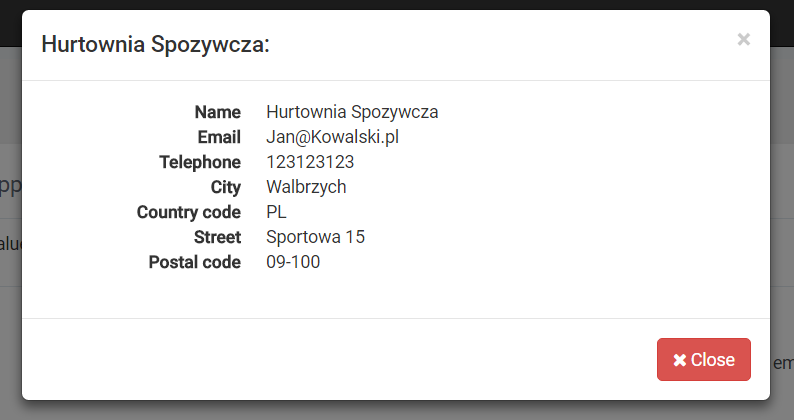
\includegraphics[width=\textwidth]{AS/supplier/3}
\end{center}
\caption{job1}
\end{figure}
\thispagestyle{empty}

\begin{figure}[h!]
\begin{center}
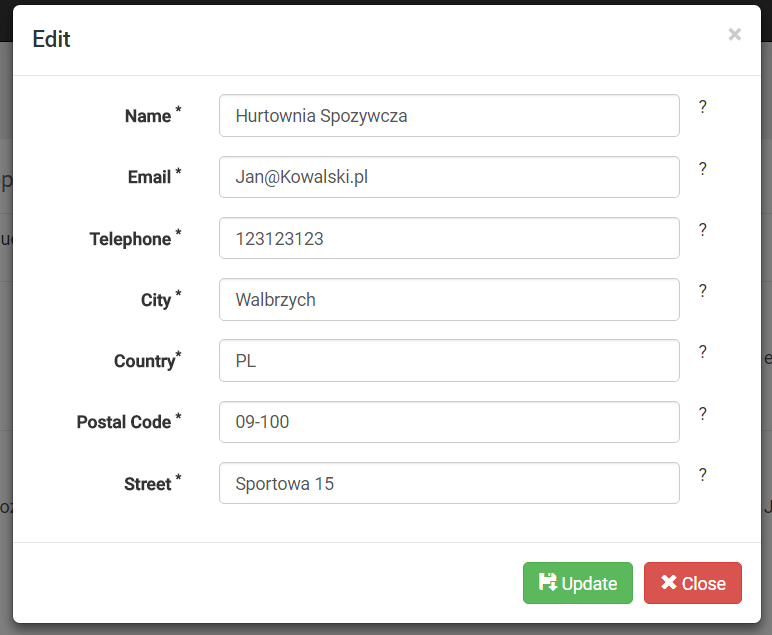
\includegraphics[width=\textwidth]{AS/supplier/4}
\end{center}
\caption{job1}
\end{figure}
\thispagestyle{empty}


\begin{figure}[h!]
\begin{center}
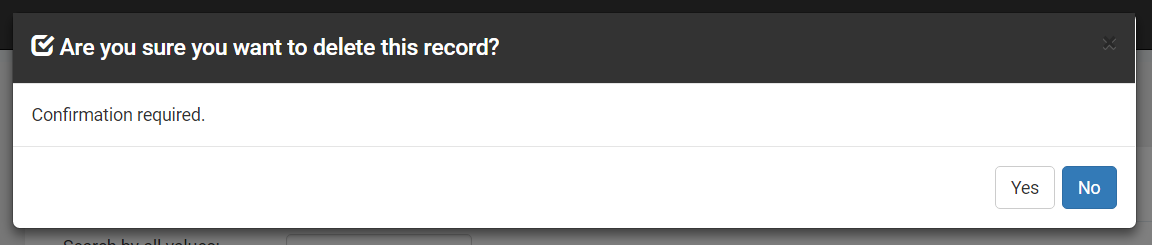
\includegraphics[width=\textwidth]{AS/supplier/5}
\end{center}
\caption{job1}
\end{figure}
\thispagestyle{empty}


\begin{figure}[h!]
\begin{center}
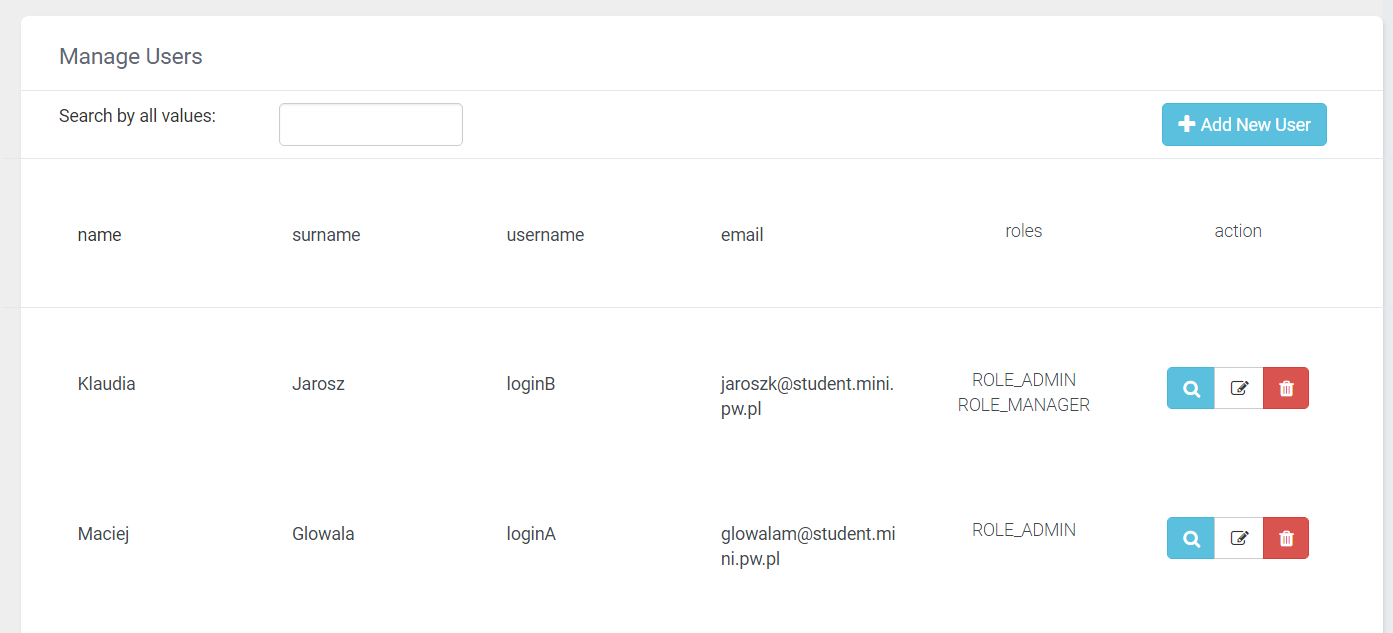
\includegraphics[width=\textwidth]{AS/users/1}
\end{center}
\caption{job1}
\end{figure}
\thispagestyle{empty}


\begin{figure}[h!]
\begin{center}
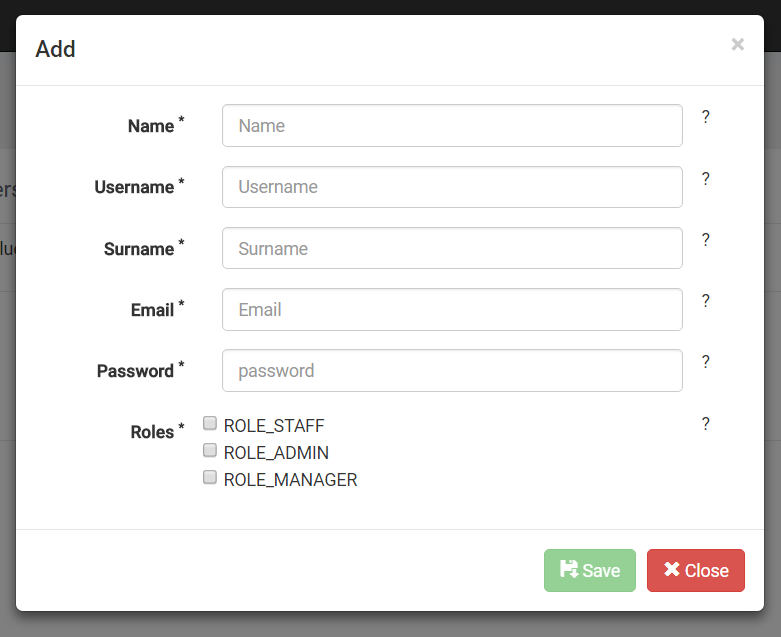
\includegraphics[width=\textwidth]{AS/users/2}
\end{center}
\caption{job1}
\end{figure}
\thispagestyle{empty}


\begin{figure}[h!]
\begin{center}
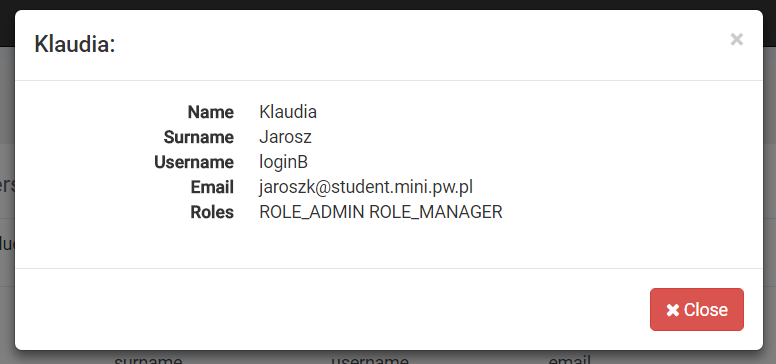
\includegraphics[width=\textwidth]{AS/users/3}
\end{center}
\caption{job1}
\end{figure}
\thispagestyle{empty}

\begin{figure}[h!]
\begin{center}
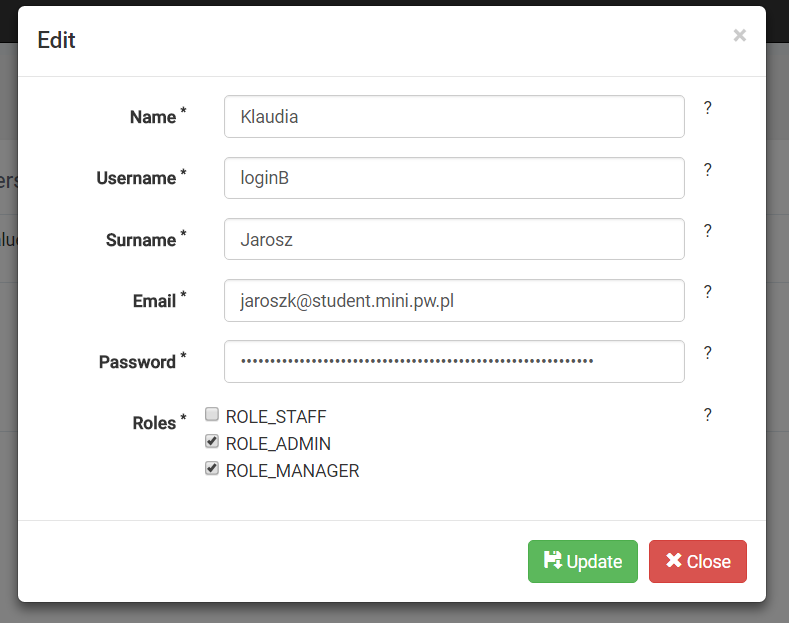
\includegraphics[width=\textwidth]{AS/users/4}
\end{center}
\caption{job1}
\end{figure}
\thispagestyle{empty}


\begin{figure}[h!]
\begin{center}
\includegraphics[width=\textwidth]{AS/users/5}
\end{center}
\caption{job1}
\end{figure}
\thispagestyle{empty}


\begin{figure}[h!]
\begin{center}
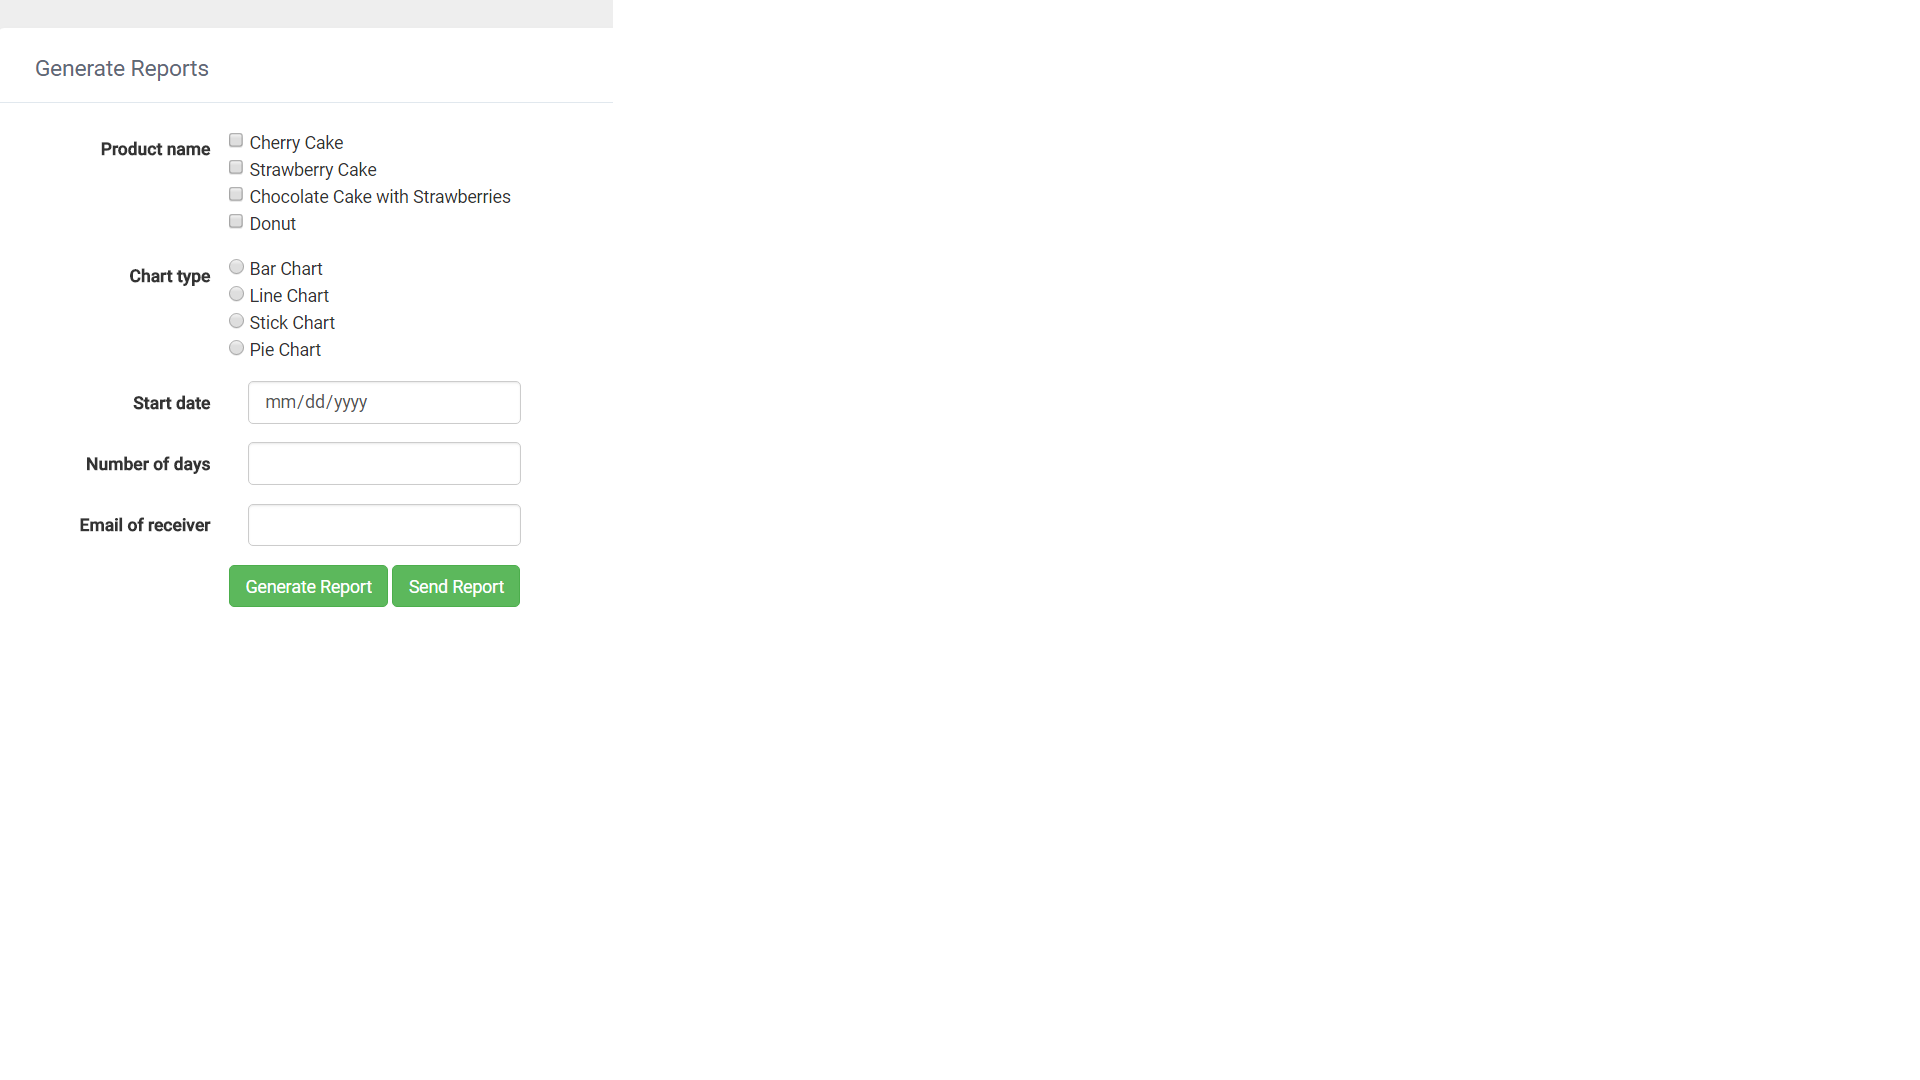
\includegraphics[width=\textwidth]{AS/report/1}
\end{center}
\caption{job1}
\end{figure}
\thispagestyle{empty}


\begin{figure}[h!]
\begin{center}
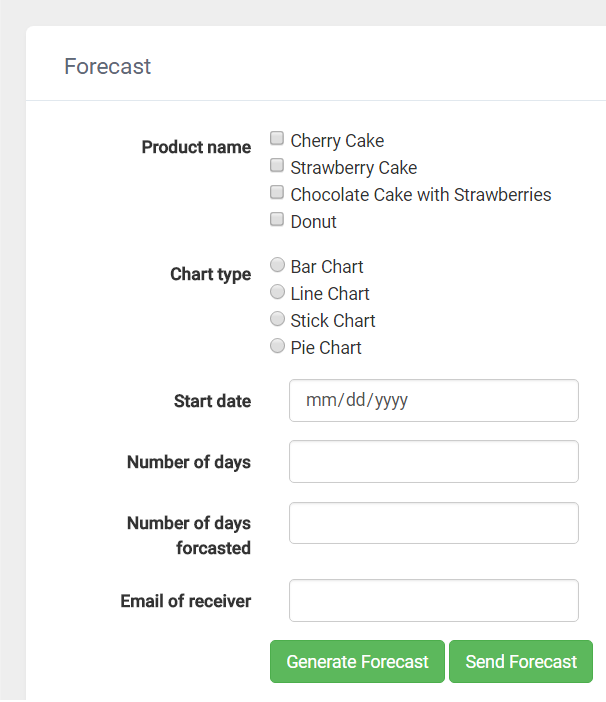
\includegraphics[width=\textwidth]{AS/report/2}
\end{center}
\caption{job1}
\end{figure}
\thispagestyle{empty}


\begin{figure}[h!]
\begin{center}
\includegraphics[width=\textwidth]{AS/report/3}
\end{center}
\caption{job1}
\end{figure}
\thispagestyle{empty}

\begin{figure}[h!]
\begin{center}
\includegraphics[width=\textwidth]{AS/report/4}
\end{center}
\caption{job1}
\end{figure}
\thispagestyle{empty}





% -----------------------------  APPENDIX B ---------------------------
\chapter*{B. Test Report}

Testi Report
\thispagestyle{empty}



\end{document}
